In the present chapter we provide the essential background material for both understanding the context of this thesis as well as the main contributions discussed in the upcoming parts.

To begin with, in Section \ref{s:basicconcepts} we briefly introduce string theory and string compactifications, focusing mostly on conceptual issues. Later on, in Sections \ref{s:maxsugraintro} and \ref{s:CYcompact} we describe the main compactification backgrounds that will be heavily employed to illustrate and study the physics presented in this thesis. In particular, we provide detailed discussions of the low energy effective actions describing the dynamics of maximally supersymmetric theories in eleven, ten, nine and eight spacetime dimensions; as well as those preserving 8 unbroken supercharges obtained from e.g., compactifying Type II string theory on Calabi--Yau manifolds. We also briefly comment in Section \ref{s:dualities} on the rich interconnections between the aforementioned theories, which arise in the form of (non-)perturbative string dualities. For a more in-depth treatment of the material presented here we refer the interested reader to the references \cite{Green:2012oqa,Green:2012pqa,Aspinwall:1996mn,Polchinski:1998rq,Polchinski:1998rr,Hori:2003ic,Becker:2006dvp,Ibanez:2012zz,Blumenhagen:2013fgp}.

Finally, to end the chapter, we introduce in Section \ref{s:SwamplandProgram} the Swampland program as well as the most important Swampland criteria that will play a starring role in this work. More concretely, we discuss in detail the Distance (Section \ref{s:SDC}) and the Weak Gravity (Section \ref{s:WGC}) conjectures. Let us mention that by now there already exists a good amount of reviews of the Swampland approach to quantum gravity \cite{Brennan:2017rbf,Palti:2019pca,vanBeest:2021lhn,Grana:2021zvf,Harlow:2022gzl,Agmon:2022thq,VanRiet:2023pnx}, which we recommend for further details on the ideas surrounding this interesting program.



\section{Basics of string theory} \label{s:basicconcepts}

The foundational premise of string theory is the conceptual replacement of point-like particles, which usually comprise the irreducible constituents in more familiar field-theoretic approaches to fundamental physics, with an entity that is additionally extended along one spatial dimension: a \emph{vibrating string}. This shift has lead to profound consequences in our understanding of the very high energy realm of Nature, uncovering fascinating phenomena that has impacted even quantum field theory itself. In this section we provide a brief introduction to the subject, highlighting the key concepts that will pay a major role in this thesis.

Crucially, unlike particles that are topologically trivial --- i.e. points without any further structure, one-dimensional objects can exhibit two inequivalent topologies: the loop (circle) and the interval (segment). Consequently, this allows for the existence of two different types of strings that can be considered within the theory: closed and open strings, respectively.

In order to describe the dynamics of relativistic strings on a $d$-dimensional spacetime $\mathcal{M}$, one usually starts from the extension of the worldline action appropriate for point-like objects, therefore adapting it to accommodate the extended nature of strings. Such a natural generalization associates an action functional to the 2d surface $\Sigma$ (i.e. the worldsheet) swept out by the string as it propagates through $\mathcal{M}$,\footnote{Note that the type of string considered, namely whether it is open or closed, is encapsulated in the topology of the worldhseet $\Sigma$ via the presence or absence of a boundary $\partial \Sigma$.} which can be locally parametrized by a set of embedding functions $X^\mu : \Sigma \to \mathcal{M}$, with $\mu=0,\dots, d-1$ and where $\sigma^a=(\tau, \sigma)$ are local coordinates on the worldsheet. It is known as the Nambu-Goto action \cite{Nambu:1986ze, Goto:1971ce}, and reads as follows
%
\begin{align}\label{eq:NambuGoto}
 S_{\text{NG}} = -\frac{1}{2\pi \alpha'} \int_\Sigma \dd^2 \sigma \sqrt{-h}\, , 
\end{align}
%
where $h$ is the (determinant of the) metric on the worldsheet induced by the one associated to the target space --- namely $g_{\mu \nu} (X)$, and $T_s$ denotes the tension of the string. The latter can be related to the more familiar string length $\ell_s=2\pi \sqrt{\alpha'}$ by $T_s=2\pi/\ell_s^2$, and it sets the energy scale beyond which non-local effects associated to the extended nature of the string must become apparent.

The action \eqref{eq:NambuGoto} captures in the most elementary way the physics of a relativistic string. Nevertheless, the explicit appearance of a square root within the 2d lagrangian formulation complicates the quantization process considerably. To address this challenge, one can benefit from the classical conformal invariance of the worldsheet theory and rewrite the Nambu-Goto action in its Polyakov version \cite{Polyakov:1981rd}, which takes the form
%
\begin{align}\label{eq:Polyakov}
 S_{\text{Poly}} = -\frac{T_s}{2} \int_\Sigma \dd^2 \sigma \sqrt{-h} h^{ab} \partial_a X^{\mu} \partial_b X^{\nu} g_{\mu \nu}\, , 
\end{align}
%
where the worldhseet metric $h_{ab}$ is now regarded as an independent field. Interestingly, eq. \eqref{eq:Polyakov} defines the perturbative string in terms of a local 2d quantum field theory living on the worldsheet, which can in principle incorporate further ingredients beyond the bosonic fields $\{X^{\mu}, h_{ab} \}$, such as fermionic superpartners $\{\psi^{\mu}, \chi_a\}$. In that case, the Polyakov action is found to be
%
\begin{equation}\label{eq:Polyakovsuperstring}
	\begin{split}
		S = & - \frac{T_s}{2} \int_\Sigma \dd^2 \sigma \sqrt{-h} \bigg(h^{ab} \partial_a X^\mu \partial_b X^\nu g_{\mu\nu} + \i \bar{\psi}^\mu \slashed{D} \psi_\mu \\ & \hspace{1cm}- 2 \i \bar{\chi}_a\rho^b\rho^a \psi^\mu \partial_b X_\mu  + \frac{1}{2}(\bar{\chi}_a\rho^b \rho^a \chi_b)(\bar{\psi}^\mu \psi_\mu)\bigg) \,,
	\end{split}
\end{equation}
%
where $\rho^a$ are two-dimensional gamma matrices satisfying the Clifford algebra (see Appendix \ref{ap:conventions} for conventions). The above action in turn defines a \emph{superstring} theory, which has many advantages over its bosonic counterpart, one of those being the incorporation of fermionic fields (from the spacetime point of view) in their quantized spectrum, which is arguably a crucial ingredient in Nature.

In fact, at the classical level, the equations of motion set the field $h_{ab}$ to be equal to the pulled-back metric from spacetime, hence recovering the Nambu-Goto action. Quantum-mechanically, however, the conformal symmetry (which is gauged in the 2d theory) can suffer from anomalies. Ensuring that this is not the case --- i.e. that the quantum string theory is consistent --- restricts the matter content as seen from the two-dimensional perspective in a non-trivial way. For instance, since the local fields in the 2d CFT are simply bosons and fermions, requiring the conformal anomaly to cancel in a flat Minkowski background $g_{\mu \nu} = \eta_{\mu \nu}$ imposes constraints on e.g., the dimension of the target spacetime, which is fixed to be $d=26$ for the bosonic string and $d=10$ for superstrings.

More importantly, when quantizing the string theory one discovers an infinite hierarchy of massive string oscillators, which may be interpreted as elementary particle excitations. In fact, separating between left-moving and right-moving modes (in the closed string case), one finds
%
\begin{subequations}\label{eq:modeexpansionclosedstring}
	\begin{align}
		X^\mu (\tau-\sigma)& = \frac12 x^{\mu} + \frac12 \alpha' p^{\mu} (\tau-\sigma) + \i\, \sqrt{\frac{\alpha'}{2}} \sum_{n\in \mathbb{Z}} \frac{1}{n} \alpha^\mu_n \, e^{-2\pi \i n (\tau-\sigma)} \,, \\[1mm]
		X^\mu (\tau+\sigma) & = \frac12 x^{\mu} + \frac12 \alpha' p^{\mu} (\tau+\sigma) + \i\, \sqrt{\frac{\alpha'}{2}} \sum_{n\in \mathbb{Z}} \frac{1}{n} \tilde{\alpha}^\mu_n \, e^{-2\pi \i n (\tau+\sigma)} \,, 
	\end{align}
\end{subequations}
%
for the bosonic fields, where $\{x^\mu, p^{\mu} \}$ are the position and momentum of the centre of mass; as well as 
%
\begin{subequations}\label{eq:fermionmodeexpansionstrings}
	\begin{align}
		\psi^\mu_L (\tau+\sigma) & = \sqrt{\alpha'} \sum_{k \in \mathbb{Z} + s} \tilde{b}^\mu_k\, e^{-2\pi \i n (\tau+\sigma)} \,, \\[2mm]
		\psi^\mu_R (\tau-\sigma) & = \sqrt{\alpha'} 	\sum_{k \in \mathbb{Z} + s} {b}^\mu_k\, e^{-2\pi \i n (\tau-\sigma)} \,,
	\end{align}
\end{subequations}	
%
for the fermionic superpartners, where $s = 0, \frac12$, accounts for Ramond (R) and Neveu--Schwarz (NS) boundary conditions, respectively.

Similarly to what happens in the worldline formalism for quantum fields, the worldsheet theory can also describe quantum interactions between string states by joining and splitting 2d surfaces, which manifest themselves via the non-trivial topology of $\Sigma$. Hence, when performing the path integral $\mathcal{Z}$ so as to derive any scattering amplitude in the theory, one is instructed to sum not only over worldsheet geometries (associated to the fluctuations of the metric $h_{ab}$) but also taking into account different topologies
%
\begin{align}\label{eq:pathintegralstring}
    \mathcal{Z}= \sum_{\rm w.s.\ topology} \int \mathcal{D}X \mathcal{D}h\, e^{ \i S_{\rm Poly}}\, .
\end{align}
%
Luckily, two-dimensional oriented real surfaces (i.e. Riemann surfaces) without boundary are completely classified at the topological level by the number of handles, namely the \emph{genus}. Hence, the formal sum over topologies in \eqref{eq:pathintegralstring} can be equivalently phrased --- in the closed string case --- as a sum over genera, and the expansion parameter controlling the series defines the string coupling constant $g_s = e^{-\phi}$, which is itself the vacuum expectation value for a dynamical field of the theory: The dilaton, see discussion around eq. \eqref{eq:RR4formfieldstrength} below.

Let us finally mention that the internal consistency of the worldsheet theory, even at the interacting level, significantly restricts the variety of viable superstring theories in ten dimensions. In fact, it has been shown that there exist precisely five distinct superstring theories in 10d, typically identified as Type I, Heterotic $\mathsf{SO(32)}$,\footnote{More correctly, such superstring theory is denoted as Heterotic $\mathsf{Spin}(32)/\mathbb{Z}_2$ \cite{Gross:1985fr}.} Heterotic $\mathsf{E8}\times \mathsf{E8}$, Type IIA, and Type IIB. These theories are distinguished by their constituents (i.e. the type of strings included and the 2d matter content) as well as the number of off-shell supersymmetries they possess: the first three have 16 unbroken supercharges (in a Minkowski background), while Type IIA and Type IIB are endowed with 32 supercharges. At low energies (compared to the string scale $m_s = \ell_s^{-1}$), the effective dynamics of the massless excitations in the aforementioned theories is described by the five existing supergravity theories in ten dimensions, see Section \ref{s:maxsugraintro} below. 


\subsubsection*{String theory compactifications}

As already argued, all five known supersymmetric string theories live naturally in ten spacetime dimensions. This does not mean, however, that there cannot exist string constructions in lower dimensions, but it suggests instead that the backgrounds we must consider should be in fact more complicated than just flat Minkowski space. This observation opens up various interesting possibilities, ranging from non-geometric constructions, where one assumes that (part of) the worldsheet theory is comprised by some intricate conformal field theory which has no direct geometric interpretation as a target Riemannian space; to geometric compactifications, where some portion of the spacetime is assumed to be compact and possibly curved.

In this thesis we follow the second route, oftentimes scanning over different effective theories that can arise from string theory when expanded over backgrounds of this sort. In what follows, we present some brief introduction to the concept of \emph{string compactifications}, so as to set up both the notation and terminology that will be heavily used in later parts of this work (see \cite{Grana:2005jc,Douglas:2023yof,Douglas:2006es} for reviews). Let us mention in passing, though, that the idea of compactification and dimensional reduction does not pertain solely to string theory, and in fact it was originally envisaged using a purely field-theoretic approach. The latter set of ideas are usually referred to as Kaluza-Klein (KK) theories, see e.g., \cite{Bailin:1987jd,Duff:1986hr} for comprehensive reviews on the topic.

Let us illustrate this point using very simple and general considerations. Thus, our aim is to find some vacuum configuration of string theory which exhibits $d$ large non-compact \emph{external} dimensions, that we assume to be flat for simplicity. In order to obtain an effective theory expanded around this background --- which is assumed to solve the equations of motion of the theory, we propose our spacetime to have (at least locally) the following product form
%
\begin{align}\label{prodansatz}
    \mathbb{R}^{1,d-1} \times X_{10-d}\, ,
\end{align}
%
where $X_{10-d}$ denotes some compact Riemannian space. To describe the physics occurring at low energies, what one can do is expand the massless spectrum of the original 10d theory using a basis of eigenfunctions of the appropriate Laplace operator $\Delta_{\rm 10}$ acting on tensor fields defined over $X_{10-d}$
%
\begin{align}
 \Delta_{10} = \Delta_{X_{10-d}} + \Delta_{d} \, .
\end{align}
%
For instance, consider the case where $X_{10-d} \cong \mathbf{S}^{10-d}$, and introduce the familiar scalar laplacian on the sphere, namely
%
\begin{align}\label{eq:scalarlaplaciansphere}
    \Delta_{\mathbf{S}^{10-d}} = \frac{1}{\sqrt{g}} \frac{\partial}{\partial \xi^i} \left( \sqrt{g} g^{ij} \frac{\partial}{\partial \xi^j}\right)\, ,
\end{align}
%
where $\{\xi^i\}$ are local coordinates on $\mathbf{S}^{10-d}$ and $g_{ij}$ defines the line element
%
\begin{align}\label{eq:lineelementsphere}
    ds^2_{10-d}= g_{ij} d\xi^i d\xi^j = \mathsf{R}^2\, d\Omega^2_{10-d}\, ,
\end{align}
%
with $\mathsf{R}$ being the radius of the sphere. Thus, given this set-up we find the corresponding eigenmodes of $\Delta$ to be given precisely by the (scalar) spherical harmonics $\mathsf{Y}_{(10-d)}^{I_1 \ldots I_\ell}$, which arise for any $\ell=0,1,\ldots$, they satisfy the condition
%
\begin{align}\label{eq:harmonics}
    -\Delta_{\mathbf{S}^{10-d}} \mathsf{Y}_{(10-d)}^{I_1 \ldots I_\ell} = \frac{\ell (\ell+9-d)}{\mathsf{R}^2} \mathsf{Y}_{(10-d)}^{I_1 \ldots I_\ell}\, ,
\end{align}
%
and are in general degenerate, with the total degeneracy of modes given by
%
\begin{align}\label{eq:deg10-dsphere}
    \frac{(9-d+2\ell)(8-d+\ell)!}{\ell! (9-d)!}\, .
\end{align}
%
The latter is precisely the number of independent components of a traceless symmetric tensor of rank $\ell$. Notice that this means, in particular, that the effective mass --- as seen from the $d$-dimensional point of view --- of any non-zero mode is controlled by the quantity $m_{\rm KK} = \frac{1}{\mathsf{R}}$, which we refer to as the Kaluza-Klein scale in here. Therefore, if we only care about energies well below $m_{\rm KK}$, it is actually more convenient to integrate out (in the path integral sense) all the massive modes and define an effective field theory (EFT) for the massless --- i.e. $\ell=0$ --- states. The process just described is what we usually understand as compactification.

A crucial question at this point is what are the type of compactification manifolds $X_{10-d}$ we can actually place our string theory on. As already mentioned, a minimal requirement would be to ask for the total ten-dimensional background \eqref{prodansatz} to solve the equations of motion in the low energy effective theory.\footnote{More appropriately, one should ask for the 2d worldsheet theory defined over such background to provide for a reliable string background, namely to exactly preserve conformal invariance.} Hence, the easiest possibility involves flat compact backgrounds --- namely tori, leading to lower-dimensional effective  theories that preserve all the original supersymmetries, since they present trivial holonomy. This possibility will be further explored in Section \ref{s:maxsugraintro} below. Another, more interesting route, would be to select non-trivial Ricci-flat manifolds which break certain amount of the supercharges but still preserve some others. This can lead ultimately to theories manifestly exhibiting 16, 8, 4 or even 0 supercharges, see Section \ref{s:CYcompact} for more on this. As an example, let us briefly discuss how to obtain four-dimensional theories preserving 8 on-shell supercharges. Starting from e.g., Type II string theory, this can be accomplished upon breaking the original holonomy group as follows $\mathsf{SO(10)} \rightarrow \mathsf{SU(2)}\times \mathsf{SU(2)} \times  \mathsf{SU(3)}$, where the last piece corresponds to the (reduced) holonomy associated to the internal dimensions. Consequently, the compact six-dimensional manifold $X_6$ we choose in \eqref{prodansatz} allows for a globally well-defined spinor $\eta(y^m)$ that is moreover covariantly constant along $X_6$, namely it satisfies
%
\begin{align}\label{eq:covariantspinor}
	\nabla_m \eta(y^m) = 0\, , 
\end{align}
%
such that the original supercharges split into the group-theoretic spinorial representation $\mathbf{16} \rightarrow (\boldsymbol{1},\boldsymbol{2},\boldsymbol{1})+ (\boldsymbol{1},\boldsymbol{1},\boldsymbol{2} )$. Therefore, every 10d Majorana-Weyl spinor $\epsilon$ gives rise to one conserved supersymmetry as follows
%
\begin{equation}\label{eq:TypeIIspinorsonCY}
\begin{split}
&\epsilon^1=\xi^1_{+} \otimes \eta_{+} + \, \mathrm{h.c.} \, ,\\
&\epsilon^2=\xi^2_{+} \otimes \eta_{-,+} +\,  \mathrm{h.c.}\, ,
\end{split}
\end{equation}
%
where $\xi^A$ are 4d Weyl spinors and the lower indices indicate their respective chiralities (depending on whether we consider the Type IIA or Type IIB string). The compact six-dimensional spaces featuring the above necessary conditions are known as Calabi--Yau manifolds, see Section \ref{ss:8supercharges} for details. 


\section{Maximally supersymmetric theories}\label{s:maxsugraintro}

A very concrete arena in which many of our discussions will take place arises from string theory compactifications preserving the maximal possible amount of supersymmetry, namely 32 supercharges. These theories can be systematically obtained from the Type IIA (or Type IIB) string on trivial compact backgrounds, i.e. tori. From a phenomenological perspective, such constructions are not very interesting, either because they live in higher dimensions or rather because they fail to exhibit the chiral spectrum that is needed to match with observations, as described by the Standard Model of Particle Physics. However, they provide a very interesting set of UV consistent quantum gravity vacua which are both computationally tractable as well as under control with regard to quantum corrections \cite{Cecotti:2015wqa}. In fact, given that the target spacetime is Riemann flat, one can quantize the Type II string \emph{exactly}, thus having access to purely stringy (or quantum gravitational) effects --- i.e. $\alpha'$ and $g_s$ corrections. %\AC{Perhaps mention non renormalisation theorems...} 

We will review here their construction as well as the features that are most relevant for the upcoming chapters. To do so, we follow an alternative route, namely we first introduce 11d supergravity, understood as the low energy limit of M-theory \cite{Witten:1995ex}, and subsequently we consider toroidal compactifications thereof. The reason is that maximal supergravity in $d\leq 9$ is unique, and can be equivalently obtained upon compactifying M-theory instead of Type II string theory, the two constructions being related by (non-perturbative) dualities, as reviewed in Section \ref{s:dualities}. We present the relevant piece of the Type IIA(B) supergravity actions in 10d, as well as their dimensionally reduced relatives in nine and eight spacetime dimensions, since they will be extensively used in Parts \ref{part:StringTheoryTests} and \ref{part:pattern} of the thesis.

\subsection{11d M-theory}\label{ss:Mthy11d}

Even though there is no fully-fledged microscopic description of M-theory as of today (see e.g., \cite{Townsend:1995kk,Banks:1996vh, Seiberg:1997ad,Nicolai:1998ic,Dasgupta:2002iy} for old attempts), one can study its dynamics at low energies --- compared with the 11d Planck scale, which is given in terms of $\mathcal{N}=1$ supergravity in eleven dimensions. The field content is completely fixed by supersymmetry \cite{Nahm:1977tg}: it contains the gravitational field $g_{\mu \nu}$, a rank-3 antisymmetric tensor $C_3$ and a Majorana gravitino $\Psi_{\mu}$, thus including a total number of 256 degrees of freedom (d.o.f.s), 128 bosonic and 128 fermionic. This theory admits a lagrangian description first obtained by Cremmer, Julia and Scherk \cite{Cremmer:1978km}, which at the two-derivative order reads as follows
%
\begin{equation}\label{eq:11daction}
    \begin{aligned}
       S_\text{M-th}^{\text{11d}} &= \frac{1}{2\kappa_{11}^2} \int \mathcal{R} \star 1 - \frac{1}{2} G_4 \wedge \star G_4 -\frac{1}{3} C_3 \wedge G_4 \wedge G_4\\
       &+\frac{1}{2\kappa_{11}^2} \int \dd^{11}x\, \sqrt{-g} \left( -2i \bar\Psi_{\mu} \Gamma^{\mu \nu \sigma} D_{\nu} \left( \frac{\omega + \hat \omega}{2}\right) \Psi_{\sigma}\right)\\
       &+ \frac{1}{2\kappa_{11}^2} \int \dd^{11}x\, \sqrt{-g}\, \frac{\i}{96} \left(\bar\Psi_{\mu_1} \Gamma^{\mu_1 \mu_2 \mu_3 \mu_4 \mu_5 \mu_6} \Psi_{\mu_2} + 12 \bar\Psi^{\mu_3} \Gamma^{\mu_4 \mu_5} \Psi^{\mu_6}\right) \left( G_4 + \hat G_4\right)_{\mu_3 \mu_4 \mu_5 \mu_6}\, ,
    \end{aligned}
\end{equation}
%
see Appendix \ref{ap:conventions} for conventions. Here $G_4=dC_3$ denotes the 4-form field strength associated to the 3-form gauge potential and $\hat G_4$ is its supercovariant counterpart, with components
%
\begin{equation}\label{eq:supercovariant4form}
       (\hat{G}_4)_{\mu_1 \mu_2 \mu_3 \mu_4} =(G_4)_{\mu_1 \mu_2 \mu_3 \mu_4} -3 \bar\Psi_{[\mu_1} \Gamma_{\mu_2 \mu_3} \Psi_{\mu_4]}\, .
\end{equation}
%
On the other hand, $D_{\nu}$ denotes the supercovariant derivative acting on the gravitino field
%
\begin{equation}\label{eq:supercovariantderivative}
       D_{\nu} \left(\omega \right) \Psi_{\sigma} = \partial_{\nu} \Psi_{\sigma} + \frac{1}{4} \omega_{\nu}^{a b} \Gamma_{a b} \Psi_{\sigma}\, ,
\end{equation}
%
where $\omega$ and $\hat \omega$ are the spin and supercovariant connections, respectively. The former is determined by the equations of motion from the action \eqref{eq:11daction} upon treating it as an independent field, whereas the latter reads as
%
\begin{equation}\label{eq:supercovariantconnection}
       \hat\omega_{\nu a b} = \omega_{\nu a b} + \frac{1}{8} \bar\Psi^{\mu} \Gamma_{\mu \nu a b \sigma} \Psi^{\sigma}\, .
\end{equation}
%
Notice that the normalization of fields other than the metric has been chosen so that the supersymmetry transformations --- under which eq. \eqref{eq:11daction} is manifestly invariant --- do not include any additional factor of the gravitational constant $\kappa_{11}$, namely
%
\begin{equation}\label{eq:11dsusyvariations}
    \begin{aligned}
       &\delta e^{a}_{\mu} = \i \bar \epsilon \Gamma^{^a}\Psi_{\mu}\, ,\\
       &\delta \Psi_{\mu} = D_{\mu} (\hat \omega) \epsilon - \frac{1}{12 \cdot 4!} \left( \Gamma^{\nu_1 \nu_2 \nu_3 \nu_4}_{\mu} + 8 \Gamma^{\nu_1 \nu_2 \nu_3} \delta ^{\nu_4}_{\mu}\right) (\hat{G}_4)_{\nu_1 \nu_2 \nu_3 \nu_4} \epsilon \, ,\\
       &\delta (C_3)_{\mu \nu \sigma} = 3 \i \bar \epsilon \Gamma_{[\mu \nu}\Psi_{\sigma]}\, ,
    \end{aligned}
\end{equation}
%
where $e^{a}_{\mu}$ is the 11d vielbein and $\epsilon(x)$ denotes any spacetime-dependent 11d Majorana spinor.

For most of our purposes here, it will be enough to focus on the bosonic part of the theory. Hence, in what follows we only display the latter when writing down any supergravity action, keeping in mind that the fermionic terms can be obtained upon completing the corresponding supermultiplets and imposing local supersymmetry, see e.g., \cite{Cecotti:2015wqa} for details on this point.

Let us also briefly comment on the massive spectrum of the theory, since we will make use of it at several instances in this work. Indeed, it is possible to argue --- either via explicit black brane solutions in 11d supergravity \cite{Gueven:1992hh} or through dualities, see Section \ref{s:dualities} below --- that the relevant BPS states admitted by the 11d supersymmetry algebra arise as electrically and magnetically charged objects under the 3-form gauge field $C_3$. These are usually referred to as M2 and M5-branes, respectively, and constitute the fundamental objects of M-theory. Their low energy dynamics is controlled by the tension and charge density of the corresponding object, and it is determined by the appropriately supersymmetrized version of the Nambu-Goto plus Chern-Simons action (see e.g., \cite{Becker:2006dvp})
%
\begin{equation}\label{eq:DBICSactionMpbranes}
				S_\text{M-brane} = -\frac{2 \pi}{\ell_{11}^{p+1}} \int_{\Sigma_{p+1}} \dd^{p+1}x\, \sqrt{- g} + \frac{2 \pi}{\ell_{11}^{p+1}} \int_{\Sigma_{p+1}}  C_{p+1}\, ,\qquad p=2, 5\, ,
\end{equation}
% 
where $\Sigma_{p+1}$ denotes the $(p+1)$-dimensional worldvolume of the associated M2 or M5-brane and $C_6$ is the magnetic dual of $C_3$.

\subsection{Type II supergravity in 10d}\label{ss:IIAB10d}

As already mentioned in Section \ref{s:basicconcepts}, conformal invariance of the 2d worldsheet theory requires that the superstring lives in ten spacetime dimensions,\footnote{Barring possible non-geometric constructions, see e.g., \cite{Gepner:1989gr,Flournoy:2004vn,Hull:2004in,Font:2017cya,Plauschinn:2018wbo} and references therein for some background on this topic.} where the minimal representation of $\mathsf{Spin(1,9)}$ is a 16-dimensional Majorana-Weyl spinor. This means that for theories with 32 supercharges, the supersymmetry generators can be arranged into two such independent spinors, with equal or different chirality (c.f. \eqref{eq:TypeIIspinorsonCY}). This partially accounts for the distinction between the two Type II string theories, which at low energies reduce to either $\mathcal{N}=(1,1)$ or $\mathcal{N}=(2,0)$ 10d supergravity, as we briefly review in the following.

\subsubsection*{Type IIA supergravity}

Let us start with non-chiral maximal supergravity in ten dimensions. This theory describes the dynamics of the massless spectrum of Type IIA string theory at energies well below the string scale. The relevant bosonic d.o.f.s consist of the metric $g_{\mu \nu}$, the Kalb-Ramond 2-form $B_2$ and the dilaton $\phi$ from the Neveu-Schwarz/Neveu-Schwarz (NSNS) sector, as well as the Ramond/Ramond (RR) $p$-forms $C_p$ with $p=1,3$. The bosonic part of the action reads in the string frame as \cite{Polchinski:1998rr}\footnote{For a more democratic formulation of the Type II string theories, whose bosonic content is extended so as to include also the magnetic $p$-form potentials along with some additional duality relations at the level of the e.o.m, see \cite{Townsend:1995gp,Bergshoeff:2001pv}.}
%
\begin{equation}\label{eq:IIA10dstringframeaction}
\begin{aligned}
S_\text{IIA, s}^{\text{10d}}\, =\, &\frac{2\pi}{\ell_s^8} \int \dd^{10}x\sqrt{-g}\ e^{-2\phi} \left(\mathcal{R}+4(\partial \phi)^2\right)-\frac{\pi}{\ell_s^8}\int e^{-2\phi} H_3\wedge \star H_3 \\
&-\frac{2\pi}{\ell_s^8}\int \left[F_2 \wedge \star F_2 + \tilde F_4 \wedge \star \tilde F_4 + B_2\wedge F_4 \wedge F_4\right]\, . 
\end{aligned}
\end{equation}
%
As is customary, $H_3=dB_2$ denotes the 3-form field strength associated to the $B_2$-field whilst $F_{p+1}$ are the field strengths of RR $p$-forms, i.e. $F_{p+1}=dC_p$. In addition, the kinetic term for the RR 3-form involves the following antisymmetric tensor 
%
\begin{align}\label{eq:RR4formfieldstrength}
 \tilde F_4 = dC_3 - C_1\wedge  H_3\, , 
\end{align}
%
which mixes with the RR 1-form and the Kalb-Ramond field due to the $\mathsf{U(1)}$ gauge invariance associated to the former. Notice that, contrary to the 11d case above, the theory has a non-trivial moduli space of vacua parametrized by the string coupling constant $g_s= e^{\phi_0}$, where $\phi_0 \equiv \braket{\phi}$ denotes the vacuum expectation value (v.e.v.) the dilaton field.

As seen from \eqref{eq:IIA10dstringframeaction}, the string frame action includes an exponential coupling to the dilaton in front of the Ricci scalar. On the other hand, whenever we want to make any (quantum) gravity statement, it is always convenient to switch to the more `canonical' Einstein frame, where the Einstein-Hilbert term is accompanied just by a constant prefactor. In the present case, this can be achieved by performing a Weyl rescaling of the form $g_{\mu \nu} \to e^{\phi/2}\, g_{\mu \nu}$, thus leading to
%
\begin{equation}
			\begin{aligned}\label{eq:IIA10dEinsteinframeaction}
				S_\text{IIA, E}^{\text{10d}} \, =\, &\frac{1}{2\kappa_{10}^2} \int \text{d}^{10}x\sqrt{-g} \left(\mathcal{R}-\frac{1}{2}(\partial \phi)^2\right)-\frac{1}{4\kappa_{10}^2}\int e^{-\phi}\, H_3\wedge \star H_3 \\
				&-\frac{1}{4\kappa_{10}^2}\int \left[e^{\frac{3}{2}\phi}\, F_2 \wedge \star F_2 + e^{\frac{1}{2}\phi}\, \tilde F_4 \wedge \star \tilde F_4 + B_2\wedge F_4 \wedge F_4\right]\, . 
			\end{aligned}
\end{equation}
%
Notice that the gravitational strength, encapsulated by the coupling constant $2\kappa_{10}^2= 2 \Mpt^{-8}= (2 \pi)^{7} \alpha'^4\ e^{2 \phi_0}$, is hence controlled by the dilaton v.e.v., which thus determines the Planck-to-string scale ratio. 

Regarding the non-perturbative massive spectrum on the theory, let us discuss now D$p$-branes. Contrary to what happened in 11d M-theory, where our only guide to deduce any possible massive excitation was supersymmetry, here there are various different ways to motivate the existence of such non-perturbative extended objects. Hence, beyond the low energy supergravity analysis, where it is possible to construct BPS black brane solutions for $p$ even \cite{Horowitz:1991cd}, one can also consider the possibility of allowing for the presence of open strings in the theory, which can end in principle on certain submanifolds $\Sigma_{p+1} \subset \mathbb{R}^{1, 9}$ \cite{Dai:1989ua,Horava:1989ga,Polchinski:1995mt} --- that supersymmetry constrain to be precisely such that $p=2k$, with $k=0,1,2,3, 4$. The inclusion of these objects breaks explicitly the 10d Lorentz symmetry, and in fact they can be viewed as $(p+1)$-dimensional states in the theory that we call D$p$-branes. Crucially, the supersymmetry algebra requires these objects to be charged under the RR $p$-forms, similarly to what happened in M-theory for the M2 and M5-branes.\footnote{Let us note that the exact same argument requires from the presence of a six-dimensional object charged magnetically under the Kalb-Ramond $B_2$-field, which is usually referred to as a NS5-brane \cite{Strominger:1990et}.}
 
A remarkable characteristic of these objects is their capacity to manifest gauge symmetries within their worldvolume theories. This ultimately arises from open strings states stretching between (possibly different) $p$-branes. In fact, it has been shown that the quantization of the open strings leads to non-trivial gauge theories living on the brane, which are described by suitable extensions of Yang-Mills theory and are frequently accompanied by additional \emph{charged} matter content. Their dynamics at low energies can be effectively described by the (supersymmetrized version of the) Dirac-Born-Infeld (DBI) action \cite{Born:1934gh, Dirac:1962iy}, which reads
%
\begin{align}\label{eq:DBITypeIIA}
S_\text{DBI} = -\frac{2\pi}{\ell_s^{p+1}} \int_{\Sigma_{p+1}} \dd^{p+1} x\ e^{-\phi} \sqrt{-\text{det} \left(g+B_2 -2\pi \alpha' \mathcal{F} \right)}\, ,
\end{align}
%
where $\mathcal{F}$ describes a field strength restricted to the worldvolume $\Sigma_{p+1}$. This action represents an extension of the Nambu-Goto action (c.f. eq. \eqref{eq:NambuGoto}), as a applied to higher-dimensional objects, and incorporates additional complexities suitable for describing the properties of D$p$-branes. Thus, upon expanding the square root of the determinant to leading order in $\mathcal{F}$ one indeed recovers (super-)Yang--Mills theory for the latter, plus an infinite number of higher-dimensional and higehr-derivative corrections in $\alpha'$. Interestingly, notice that quantizing the worldvolume theory of the D$p$-branes in a similar manner to what we did for the fundamental string in Section \ref{s:basicconcepts}, is strictly speaking not possible, since the theory \eqref{eq:DBITypeIIA} is not conformally invariant, such that it cannot be recasted in the Polyakov form. Let us also note that the DBI action includes an additional coupling to the dilaton, which implies that the physical tension of the branes grow like $g_s^{-1}$, thus suggesting that they are actually non-perturbative in nature, at least from the string theory point of view. 

On the other hand, the interaction between the D-branes and the RR $p$-forms is determined by the Chern--Simons (or Wess--Zumino) action 
%
\begin{align}\label{eq:CSWZactionTypeIIA}
S_\text{CS} = \frac{2\pi}{\ell_s^{p+1}} \int_{\Sigma_{p+1}} \left(\sum_q C_q \right) \wedge e^{2\pi \alpha' \mathcal{F} -B_2} \wedge \sqrt{\frac{\hat A (\ell_s^2 \mathcal{R}_T)}{\hat A (\ell_s^2 \mathcal{R}_N)}}\, ,
\end{align}
%
where the ${\text{A}}$-roof genus depends on the curvature 2-forms $\mathcal{R}_T$ and $\mathcal{R}_N$ of the tangent and normal bundles (respectively) of $\Sigma_{p+1}$ as follows 
%
\begin{align}
\hat A \left(\ell_s^2 \mathcal{R}_{N(T)} \right) = \frac{1}{(2\pi)^{\frac{p+1}{2}}} \sqrt{\det \left( \frac{\ell_s^2 \mathcal{R}_{N(T)}/2}{\sinh \left( \ell_s^2 \mathcal{R}_{N(T)}/2\right)}\right)}\, .
\end{align}
%
Therefore, depending on the topology and geometry of $\Sigma_{p+1}$, there can appear induced lower $q$-form charges on the D$p$-brane, see e.g., \cite{Witten:1998cd}. 

\subsubsection*{Type IIB supergravity}

Type IIB String Theory presents a chiral spectrum, such that at energies well below the string sale it reduces to 10d $\mathcal{N}=(2,0)$ supergravity in ten dimensions. The bosonic fields in the NSNS sector agree with those of Type IIA string theory, whilst the RR one provides for a different set of $p$-form gauge fields, namely $C_p$ with $p=0,2,4$. The 4-form $C_4$ has moreover a self-dual field strength satisfying $\tilde F_5= \star \tilde F_5$, and the dynamics (i.e. equations of motion) of the theory can be encapsulated (at the two derivative level) by the following pseudo-action \cite{Polchinski:1998rr} 
%
\begin{equation}\label{eq:IIB10d}
			\begin{aligned}
				S_\text{IIB}^{\text{10d}}\, =\, & \frac{1}{2\kappa_{10}^2} \int \dd^{10}x\sqrt{-g} \left(\mathcal{R}-\frac{1}{2}(\partial \phi)^2\right) -\frac{1}{4\kappa_{10}^2}\int e^{-\phi} H_3\wedge \star H_3 \\
				&-\frac{1}{4\kappa_{10}^2}\int \left[e^{2 \phi}F_1 \wedge \star F_1 + e^{\phi} \tilde F_3 \wedge \star \tilde F_3 + \frac{1}{2} \tilde F_5 \wedge \star \tilde F_5  +C_4\wedge H_3 \wedge F_3\right]\,,
			\end{aligned}
\end{equation}
%
where we have already switched to the Einstein frame upon performing the same Weyl rescaling as in Type IIA. The different field strengths are defined as follows
%
\begin{equation}
\begin{aligned}
&H_3=dB_2\, , \qquad  \tilde{F}_3=dC_2-C_0 H_3\, ,\\
&F_1=d C_0\, , \qquad \tilde{F}_5= dC_4-\frac{1}{2} C_2 \wedge F_3 + \frac{1}{2} B_2 \wedge H_3\, . 
\end{aligned}
\end{equation}
%
Analogously to the Type IIA case, the existence of exactly massless scalar fields in the theory --- i.e. the dilaton and the axion $C_0$, implies that there is a non-trivial moduli space (of complex dimension one) parametrized by the former. Several features of such moduli space will be discussed later on in Section \ref{s:dualities} and exploited in the rest of this thesis.

Finally, let us turn to the D-brane spectrum of the theory. Notice that, since the RR field content is different for Type IIB string theory, the possible extended objects saturating the BPS conditions can become quite distinct. Indeed, following the same logic as outlined before, one finds a D$(-1)$-brane --- i.e. an instanton --- coupling electrically to $C_0$, a D1-string coupling electrically to $C_2$, and a D3-brane coupled to the self-dual 4-form, together with their magnetic duals: the D5 and the D7-branes. Again, their stability is ensured by supersymmetry and the low energy dynamics is described in terms of the DBI and Chern--Simons actions, c.f. eqs. \eqref{eq:DBITypeIIA} and \eqref{eq:CSWZactionTypeIIA}. 

\subsection{Maximal supergravity in 9d}\label{ss:9dmaxsugra}

In nine dimensions there is a unique theory of gravity with 32 supercharges, namely 9d $\mathcal{N}=2$ supergravity \cite{Gates:1984kr}. It can be easily obtained from any of the previous 10d Type II supergravities after dimensionally reducing on a circle $\mathbf{S}^1$, which washes away the original chirality distinction in ten dimensions. Alternatively, if we only care about the low energy lagrangian description, it is equivalent (up to field redefinitions) to start from 11d $\mathcal{N}=1$ supergravity and compactify two spatial directions on a torus $\mathbf{T}^2$. Here we choose this second route for convenience. Of course, ultimately the fact that the 9d theory can be retrieved from any of these corners of the string theory landscape is simply a manifestation of the intricate dualities relating the aforementioned descriptions (see Section \ref{s:dualities} below). 

Hence, we consider M-theory at low energies, described by the action \eqref{eq:11daction} and we impose the following ansatz for the 11d metric 
%
\begin{equation}\label{eq:11dmetric}
	ds^2_{11} = \mathcal{V}_2^{-2/7} ds_9^2 + \mathcal{V}_2 \left( \tau_2^{-1}\left( dy^1- A_1^{(1)}+\tau_1 dy^2\right)^2+ \tau_2\left( dy^2 - A_1^{(2)}\right)^2\right)\, ,
\end{equation}
%
where the fields $A^{(i)}_1$ are Kaluza-Klein 1-forms in the non-compact 9d space. Notice that the purely internal piece of the above line element can be written as
%
\begin{equation}
	ds^2_{\mathbf{T}^2}= g_{mn} dy^m dy^n\, , \qquad \text{with}\quad g_{mn}= \frac{\mathcal{V}_2}{\tau_2} \left(
	\begin{array}{cc}
		1 & \tau_1  \\
		\tau_1 & |\tau|^2  \\
	\end{array}
	\right) \, ,
\end{equation}
%
with $\tau=\tau_1+{\rm i}\tau_2$ being the complex structure of the torus and $\mathcal{V}_2$ denoting its overall volume (in M-theory units). After doing so, one obtains
%
\begin{equation}\label{eq:9daction}
\begin{aligned}
    S_\text{M-th}^{\text{9d}} &= \frac{1}{2\kappa_9^2} \int \dd^{9}x\, \sqrt{-g}\,  \left( \mathcal{R} - \frac{9}{14} \left( \partial \log \mathcal{V}_2 \right)^2 -\frac{\partial \tau \partial \bar \tau}{2 \tau_2^2} \right) - \frac{1}{4\kappa_9^2} \int \frac{\mathcal{V}_2^{9/7}}{\text{Im}\, \tau}F_2 \wedge \star \bar{F}_2\\
    & - \frac{1}{4\kappa_9^2} \int \mathcal{V}_2^{-12/7} dC_1 \wedge \star dC_1+\frac{\mathcal{V}_2^{4/7}}{\text{Im}\, \tau}F_3 \wedge \star \bar{F}_3 + \mathcal{V}_2^{3/7}dC_3 \wedge \star dC_3\\
    & - \frac{1}{2\kappa_9^2} \int C_1 \wedge dC_3 \wedge dC_3\, ,
\end{aligned}
\end{equation}
%
where we have absorbed an overall volume factor into the 9d gravitational coupling constant.\footnote{\label{fnote:11d-9dPlancklengths}More precisely, the 11d and 9d Planck lengths are related by $\ell_{11}^7=\ell_9^7\, \mathcal{V}_2$, see Appendix \ref{ap:conventions} for conventions.} The nine-dimensional bosonic fields other than the metric arrange into a scalar sector $\{ \mathcal{V}_2, \tau\}$ parametrizing the vacuum manifold; the two KK 1-forms with a complex field strength defined by $F_2= dA^{(1)}_1- \tau dA^{(2)}_1$, as well as an additional 1-form $C_1$ obtained from the reduction of the 11d 3-form on the torus; a complex 2-form with field strength $F_3= dC^{(1)}_2- \tau dC^{(2)}_2$ arising from the 11d 3-form with one leg along any internal direction; and a single 3-form gauge field $C_3$.

Before moving on, let us mention that the moduli space of the 9d theory can be seen to be isomorphic to the group coset $\mathcal{M}_{\text{9d}}=\mathbb{R}_+ \times \mathsf{SL(2, \mathbb{R})}/\mathsf{SO(2)}$, where the first factor corresponds to the torus volume and the second one is identified with its complex structure. To see this, one first defines a moduli-dependent upper triangular matrix as follows
%
\begin{equation}\label{eq:Pmatrix}
	\mathcal{P} = \left( \begin{array}{cc}
		\tau_2^{-1/2} & \tau_1 \tau_2^{-1/2} \\
		0 & \tau_2^{1/2}  \\
	\end{array}
	\right) \, ,
\end{equation}
%
as well as the symmetric $2\times 2$ matrices $\mathcal{Q} = \mathcal{P}^{\text{T}} \mathcal{P}$ and its inverse $\mathcal{Q}^{-1}$
%
\begin{equation}
	\mathcal{Q} = \left( \begin{array}{cc}
		\tau_2^{-1} & \tau_1 \tau_2^{-1} \\
		\tau_1 \tau_2^{-1} & \tau_2 + \tau_2^{-1} \tau_1^2  \\
	\end{array}
	\right) \, , \qquad 
   \mathcal{Q}^{-1} = \left( \begin{array}{cc}
		 \tau_2 + \tau_2^{-1} \tau_1^2 & -\tau_1 \tau_2^{-1} \\
		-\tau_1 \tau_2^{-1} & \tau_2^{-1}  \\
	\end{array} \right)\, ,
\end{equation}
%
which both have unit determinant. Using these objects, the complex structure piece of the 9d lagrangian can be written in matrix form as
%
\begin{equation}\label{eq:sl2matrixform}
	-\frac{1}{2 \tau_2^2} \partial \tau \cdot \partial \bar \tau= \frac{1}{4} \text{tr}\, \left( \partial\mathcal{Q}^{-1} \cdot \partial \mathcal{Q} \right)\, .
\end{equation}
%
Therefore, one may alternatively describe the 9d moduli space in terms of unimodular matrices of the upper triangular form displayed in \eqref{eq:Pmatrix}. In addition, notice that under generic $\mathsf{SL(2, \mathbb{R})}$ transformations acting from the right on $\mathcal{P}$, one finds that $\mathcal{Q} \to \mathcal{A}^{\text{T}} \mathcal{Q} \mathcal{A}$, with $\mathcal{A} \in \mathsf{SL(2, \mathbb{R})}$. These transformations thus leave invariant the kinetic term \eqref{eq:sl2matrixform}, preserving moreover the unimodular condition. However, they do not, in general, maintain the upper triangular form of $\mathcal{P}$. Upon further accounting for such `compensating' $\mathsf{SO(2)}$ rotations one concludes that the complex modulus $\tau$ can be equivalently described by the group of $\mathsf{SL(2, \mathbb{R})}$ matrices up to 2d rotations, as claimed. In fact, at the classical level, one can easily get convinced that the action \eqref{eq:9daction} above is symmetric under the group $\mathsf{SL(2, \mathbb{R})}$, with scalars transforming as indicated above whilst the different $p$-forms transform linearly, either as a doublet (the complex 1- and 2-forms $F_2$, $F_3$) or as a singlet ($C_1$ and $C_3$).

Regarding the massive spectrum of the theory, it can be deduced directly from that of the parent 11d description, as will be explained in more detail in Section \ref{ss:MthyT2SSDC}, so that we refrain from repeating it here and refer the interested reader to Chapter \ref{ch:bounds} of the thesis.

\subsection{Maximal supergravity in 8d}\label{ss:8dmaxsugra}

Following the analysis of the previous section, a good strategy to obtain the maximal supergravity action for a given spacetime dimension $d\leq 9$ is to consider M-theory compactified on a $k=11-d$ dimensional torus, with a metric ansatz of the form 
%
\begin{equation}\label{eq:torusmetric}
	ds^2_{11} = \left(\text{det}\, g_{mn}\right)^{-\frac{1}{d-2}} ds_d^2 + g_{mn} dy^m dy^n\, .
\end{equation}
%
where $g_{mn}$ parametrizes the metric on the internal torus. As usual, the prefactor in the $d$-dimensional line element has been chosen so as to obtain the resulting lower dimensional theory in the Einstein frame. Therefore, in order to find the correct description of maximal supergravity in eight dimensions one simply needs to compactify M-theory on $\mathbf{T}^3$.

Notice that we did not include in \eqref{eq:torusmetric} the fluctuations in the metric associated to the Kaluza-Klein photons (c.f. eq. \eqref{eq:11dmetric}). The reason for this is because we will focus in this section solely on the gravitational-scalar sector of the theory, thus forgetting about any other tensorial field, since it will play no role in the analysis performed in the upcoming chapters (see \cite{Salam:1984ft} for the full supersymmetric action). After these manipulations, one finally arrives at
%
\begin{align}\label{eq:8dsl3}
	S_\text{M-th}^{\text{8d}}\, \supset\, &\frac{1}{2\kappa_8^2} \int \dd^{8}x\, \sqrt{-g}\,  \left( \mathcal{R} + \frac{1}{4} \text{tr} \left( \partial \tilde{g} \cdot \partial \tilde{g}^{-1} \right) -\frac{\partial \mathcal{T} \cdot \partial \bar{\mathcal{T}}}{2 \mathcal{T}_2^2} \right)\, ,
\end{align}
%
where the $3\times3$ matrix $\tilde{g}$ is obtained from the internal metric of the $\mathbf{T}^3$ with the overall volume extracted, i.e. $\tilde{g}_{m n}= \mathcal{V}_3^{-2/3} g_{mn}$. More precisely it reads as
%
\begin{align}\label{eq:trace8d}
	-\text{tr} \left( \partial \tilde{g} \cdot \partial \tilde{g}^{-1} \right) = \left(\tilde{g}^{m p} \tilde{g}^{n q}+ \frac{1}{6} \tilde{g}^{mn} \tilde{g}^{pq} \right) \partial \tilde{g}_{mn} \cdot \partial \tilde{g}_{pq}\, .
\end{align}
%
In addition, we have defined the complex field $\mathcal{T}=C_{123}^{(3)} + \text{i} \mathcal{V}_3$, which contains the compact scalar $C_{123}^{(3)}$ arising from the reduction of the 11d 3-form $C_3$ along the torus as well as the volume modulus. Note that the parametrization in \eqref{eq:8dsl3} is rather useful since it already makes manifest certain symmetries of the classical action. In fact, to detect those it is enough to realize that the moduli $\{ \tilde{g}_{m n}, \mathcal{T}\}$, parametrize the coset space\footnote{One quick way to understand the $\mathsf{SL(3, \mathbb{R})}$ symmetry of the action \eqref{eq:8dsl3} is by realizing that the fields $\tilde g_{mn}$ transform in the adjoint representation, namely $\tilde g \to \mathcal{A}^{\text{T}} \tilde g \mathcal{A}$, with $\mathcal{A} \in \mathsf{SL(3, \mathbb{R})}$. Such transformations thus leave the trace \eqref{eq:trace8d} invariant.}
%
\begin{align}
	\mathcal{M}_{\text{8d}} = \frac{\mathsf{SL(3, \mathbb{R})}}{\mathsf{SO(3)}} \times \frac{\mathsf{SL(2, \mathbb{R})}}{\mathsf{SO(2)}}\, ,
\end{align}
%
which exhibits some nice structure that will play an important role in Parts \ref{part:StringTheoryTests} and \ref{part:pattern} of the thesis.

For future reference, it is also convenient to rewrite \eqref{eq:8dsl3} using an alternative set of fields that arise more naturally when directly reducing the 9d action introduced in Section \ref{ss:9dmaxsugra} above, on $\mathbf{S}^1$. Therefore, starting from eq. \eqref{eq:9daction} and upon further compactification on a circle of radius $R_3$ (measured in 9d Planck units), we find
%
\begin{equation}\label{eq:8dalternativeaction}
\begin{aligned}
	S_\text{M-th}^{\text{8d}}\, &\supset\, \frac{1}{2\kappa_{8}^2} \int \dd^{8}x\sqrt{-g} \Bigg[\mathcal{R}-\frac{9}{14} \left( \partial \log \mathcal{V}_2\right)^2 - \frac{7}{6} \left( \partial \log R_3\right)^2 -\frac{\partial \tau \cdot \partial \bar \tau}{2 \tau_2^2}\\
      &- \frac{\mathcal{V}_2^{-12/7} R_3^{-2}}{2} \left( \partial C_{123}^{(3)}\right)^2 -\frac{\mathcal{V}_2^{9/7} R_3^{-2}}{2 \tau_2} \left| \partial A^{(1)}_0-\tau \partial A^{(1)}_0 \right|^2\Bigg]\, ,
\end{aligned}
\end{equation}
%
where $C_{123}^{(3)}$ is defined after eq. \eqref{eq:trace8d} and the compact scalars $\{ A^{(1)}_0, A^{(1)}_0 \}$ parametrize the orientation of the two-dimensional torus within the $\mathbf{T}^3$. From the parent nine-dimensional theory, these arise from the reduction of the singlet and doublet of 1-forms along the extra circle, see discussion around after eq. \eqref{eq:9daction}. Moreover, the overall $\mathbf{T}^3$ volume can be expressed in terms of those of the submanifolds $\mathbf{T}^2$ and $\mathbf{S}^1$ as follows
%
\begin{equation} \label{eq:T3volume}
     \mathcal{V}_3 = \mathcal{V}_2\, R_3\, \frac{\ell_9}{\ell_{11}} = \mathcal{V}_2^{6/7}\, R_3\, ,
\end{equation}
%
where the relation between the 9d and 11d Planck lengths can be found in footnote \ref{fnote:11d-9dPlancklengths}.

Let us conclude by mentioning that the (non-)perturbative massive spectrum of the present 8d theory will be discussed in more detail in Section \ref{ss:MthyT3SSDC} (see in particular Table \ref{tab:BPSstates}), to which we refer in here.

\section{Theories with reduced supersymmetry}\label{s:CYcompact}

In this section we proceed by introducing and discussing effective field theories in diverse spacetime dimensions which preserve less amount of supersymmetry. In particular, we focus on EFTs that exhibit either 16 (Section \ref{ss:16supercharges}) or 8 unbroken supercharges (Section \ref{ss:8supercharges}). They are less constrained than their maximally supersymmetric counterparts, which already implies that there can be significant quantum corrections (both perturbative and non-perturbative), even at the two-derivative level. On the other hand, they exhibit rich dynamics accommodating for further ingredients that are moreover phenomenologically attractive. We have chosen certain representative examples in each case, based on the analysis carried in later parts of the thesis.

\subsection{Compactifications preserving 16 supercharges} \label{ss:16supercharges}

There are in fact many ways to obtain low energy effective theories preserving 16 supercharges. One economic way to do so is to start from (any of) the Heterotic string(s) --- or Type I string theory --- in ten spacetime dimensions, which precisely exhibit that amount of supersymmetries, and subsequently reduce the theory on flat tori. This already provides for various interesting phenomena that are absent in maximally supersymmetric constructions, such as gauge enhancements at special points in moduli space (see \cite{Font:2020rsk} for a recent analysis of this family of string theory compactifications). Even though we will utilize these theories to illustrate some of the physics described in this work (see in particular Section \ref{ss:het s1} below), we refrain from presenting here a detailed analysis of their low energy dynamics. Instead, we have chosen to describe another set-up preserving 16 supercharges which arises from M-theory compactifications on $K3$ surfaces, since it also appears at several instances in the thesis, playing a major role in our discussions.

%\subsubsection{Heterotic string theory on $\mathbf{S}^1$}\label{sss:HeteroticonS1}

%\AC{To be written}

\subsubsection{M-theory on a $K3$ surface}\label{sss:MtheoryonK3}

Let us consider M-theory compactified on a $K3$ manifold down to seven (non-compact) spacetime dimensions. The resulting theory displays (minimal) $\mathcal{N}=1$ supersymmetry in 7d, namely it preserves 16 of the original 32 supercharges of 11d supergravity. In fact, a useful way to think about $K3$ is in terms of a $\mathbf{T}^4/\mathbb{Z}_2$ orbifold, where the discrete group acts as $z^i \to -z^i$ on the two complex coordinates parametrizing the torus. The $\mathbb{Z}_2$ group acts non-freely, such that there are 16 fixed points in total which locally look like $\mathbf{R}^4/\mathbb{Z}_2$, that are responsible for breaking half of the original supersymmetries. One can moreover associate 3 parameters to each of these points, which can be used to resolve the singularity into some $\mathbb{P}^1$ blow-up, thus leaving some smooth space behind of the Eguchi-Hanson type \cite{Eguchi:1978gw}
%
\beq\label{eq:EguchiHanson}
	ds^2_{\rm{EH}}= f(r)^{-1}dr^2+r^2 f(r) \left( d\psi + \cos \theta d\phi \right)^2 + r^2 \left( d\theta^2 + \sin^2 \theta d\phi^2\right)\, ,
\eeq
%
with $f(r)=1-\left(\frac{t}{r}\right)^4$ and where $(\theta, \phi, \psi)$ parametrize a 3-sphere (modded out by $\mathbb{Z}_2$ due to the identification $\psi \sim \psi + 2\pi$). The free parameters correspond to $t$, which provides the size of the 2-cycle, together with two additional angles that control the orientation of the $\mathbb{P}^1$ inside $\mathbb{R}^4$. 

Here we will only need to know a few topological and geometric facts that are specific to $K3$ manifolds (see e.g., \cite{Aspinwall:1996mn} for more details).\footnote{In the mathematical literature, $K3$ surfaces are defined as compact K\"ahler manifolds of complex dimension two with vanishing first Chern class. Therefore, they are nothing but Calabi--Yau two-folds, see Section \ref{ss:8supercharges} below.} First, for a given complex structure, the Hodge decomposition of $H^2(K3, \mathbb{R})$ is such that the Hodge numbers read
%
\beq\label{eq:hodgeK3}
	h^{2,0}(K3) = h^{0,2}(K3) = 1\,,\qquad h^{1,1}(K3) = 20\, .
\eeq
%
To these we can associate a basis of harmonic 2-forms, i.e. $\lbrace \omega_A \rbrace= \lbrace \Omega_2, \overline \Omega_2, \omega_a \rbrace$, where $\Omega_2 \in H^{2,0}(K3)$ is the unique holomorphic (2,0)-form and $\omega_a \in H^{1,1}(K3)$, $a=1, \ldots, h^{1,1}(K3)$. In addition, the Hodge star operator maps $H^2(K3, \mathbb{R})$ to itself, and moreover satisfies $\star^2=1$. Therefore, one may divide the second cohomology group of $K3$ into self-dual and anti self-dual  forms, namely $H^2(K3, \mathbb{R}) = H_+^2(K3, \mathbb{R}) \oplus H_-^2(K3, \mathbb{R})$, where $\dim H_+^2(K3, \mathbb{R})=3$ and $H_-^2(K3, \mathbb{R})=19$. The former admits a natural basis spanned by the real and imaginary parts of $\Omega_2$, together with the K\"ahler 2-form $J= t^a \omega_a$, which controls the volume of the different holomorphic cycles within the $K3$. 
		
With the above mathematical background, we are now ready to discuss both the field content and the low energy dynamics of the resulting theory. In a supersymmetric language, one is left with $d=7$, $\mathcal{N}=1$ supergravity coupled to 19 abelian vector multiplets (at generic points in moduli space). The gravity multiplet contains the metric field, a 2-form (which can be dualized to a 3-form gauge field in 7d), an $\mathsf{SO(3)}$ triplet of 1-forms and a scalar field. On the other hand, each vector multiplet consists of a 1-form potential as well as an $\mathsf{SO(3)}$ triplet of scalar fields. The scalar sector arises from the deformations of the $K3$ metric, which comprise 58 parameters in total, one of which corresponding to the overall volume --- which belongs to the gravity multiplet.\footnote{In the orbifold description, the scalar fields arise from the internal metric of the $\mathbf{T}^4$ (10 in total) together with each of the 3 parameters associated to the 16 fixed points (48 scalars).} Finally, the 3-form and 1-forms both descend from the 11d 3-form field $C_3$:
%
\beq\label{eq:7dreductionC3}
		C_3=A^a \wedge \omega_a + A_3\, .
\eeq
%
Notice that the latter arise upon reducing $C_3$ on a basis of harmonic 2-forms in $K3$. One thus obtains $h^2(K3)=22$ 1-form gauge potentials in total, three of which belong to the gravity multiplet.

All in all, the relevant piece of the 7d (bosonic) action reads as follows
%
\begin{equation}\label{eq:7dMthyK3}
	\begin{aligned}
		S_\text{M-th}^{\text{7d}}\, =\, & \frac{1}{2\kappa^2_7} \int \dd^{7}x\, \sqrt{-g}\,  \left( \mathcal{R} - \frac{9}{20} \left( \partial \log \mathcal{V}_{K3} \right)^2 - G_{i j} \partial \phi^i \cdot \partial \phi^j\right)\\
        &  -\frac{1}{4\kappa_{7}^2} \int \mathcal{V}_{K3}^{6/5}\, dA_3 \wedge \star dA_3 + \mathcal{V}_{K3}^{-3/5} \mathsf{G}_{a b} F^a \wedge F^b + 2\eta_{a b} A_3 \wedge F^a \wedge F^b\, ,
	\end{aligned}
\end{equation}
%
where $\mathcal{V}_{K3} = \frac{1}{2} \eta_{ab} t^a t^b$ is the overall volume of the internal space and $\eta_{ab}= \omega_a \cdot \omega_b \equiv \int_{K3} \omega_a \wedge \omega_b$ denotes the intersection form of the $K3$ surface. The fields $\phi^i$, $i=1, \ldots, 57$, parametrize the vector multiplet moduli space, i.e. the space of deformations of Ricci-flat K\"ahler metrics on $K3$ with fixed overall volume. This is given by the group coset \cite{Aspinwall:1996mn}
%
\begin{align}\label{eq:cosetspace7d}
	\mathcal{M}_{\text{VM}} = \mathsf{O(\Gamma_{3,19})}\backslash \mathsf{O(3,19)} / (\mathsf{O(3)} \times \mathsf{O(19))}\, ,
\end{align}
%
where $\Gamma_{3,19}$ denotes the lattice with signature $(3,19)$ that is isomorphic to the integer (non-trivial) cohomology on K3. The tensor $G_{ij}$ is the canonical metric on $\mathcal{M}_{\text{VM}}$, whose explicit form can be found in the original references, see \cite{Duff:1983vj}. On the other hand, the gauge kinetic matrix for the vectors depends solely on the K\"ahler deformations through the functions $\mathsf{G}_{a b}$. Its explicit form can be readily computed to be \cite{Lee:2019xtm}
%
\begin{equation}\label{eq:7dmodspacemetric}
	\begin{aligned}
		\mathsf{G}_{a b} = \int_{K3} \omega_a \wedge \star \omega_b = \frac{t_a t_b}{\mathcal{V}_{K3}}- \eta_{a b} = \tilde{t}_a \tilde{t}_b -\eta_{a b}\, ,
	\end{aligned}
\end{equation}
%
where the indices are lowered with the intersection form $\eta_{a b}$. In addition, one can argue that the action \eqref{eq:7dMthyK3} is classically exact \cite{Witten:1995ex, Cadavid:1995bk} and hence does not receive any further quantum corrections. This is in contrast to e.g., Type IIA string theory on the same two-fold, which probes the quantum $H^2(K3)$-cohomology due to the extra modes arising from the $B_2$-field.

An important simplification occurs when the $K3$ surface is \emph{attractive} \cite{Moore:1998pn}, namely when the rank of its Picard group is maximal.\footnote{The Picard group is defined as $\text{Pic}(K3)= H^{1,1}(K3) \cap H^2(K3,\mathbb{Z})$, such that it corresponds to (dual) curve classes which have some holomorphic representative \cite{Aspinwall:1996mn}. For attractive $K3$ two-folds, $\text{rk}(\text{Pic}(K3))=20$.} For such manifolds, the complex structure is completely fixed (see e.g., \cite{Moore:1998zu} for details on this), so that both the 7d lagrangian as well as the mass of the different (non-)perturbative states depend solely on the K\"ahler moduli. In those cases, the scalar lagrangian in \eqref{eq:7dMthyK3} reduces to
%
\begin{equation}\label{eq:7dMthyattractive}
	\begin{aligned}
		\mathcal{L}_\text{M-th}^{\text{7d}}\, \supset\, - \frac{1}{2\kappa^2_7} \sqrt{-g}\,  \left[ \frac{9}{20} \left(\frac{\partial \mathcal{V}_{K3}}{\mathcal{V}_{K3}} \right)^2 + \mathsf{G}_{a b}\, \partial \tilde{t}^a \cdot \partial \tilde{t}^b \right]\, ,
	\end{aligned}
\end{equation}
%
where $\tilde{t}^a= t^a/\mathcal{V}_{K3}^{1/2}$ are rescaled moduli subject to the constraint $ \frac{1}{2} \eta_{ab} \tilde{t}^a \tilde{t}^b \stackrel{!}{=} 1$ and $\mathsf{G}_{a b}$ is given in \eqref{eq:7dmodspacemetric}. 


\subsection{Compactifications preserving 8 supercharges} \label{ss:8supercharges}

We finally turn to theories preserving $1/4$ or $1/2$ of the original supersymmetries, depending on whether they arise from Type II or Heterotic string compactifications. Their significance within the context of the present thesis lies in the fact that whilst they are still under computational control, the dynamics is far richer than their higher supersymmetric cousins --- even at the two-derivative level. In fact, the geometry of their moduli spaces can receive a plethora of quantum and stringy corrections, which can be then used to learn non-trivial aspects of (non-)perturbative quantum gravity. 

In this subsection we will particularize to two sets of theories preserving eight unbroken supercharges, which live in four and five non-compact spacetime dimensions. These set-ups can be obtained upon compactifying e.g., Type II string theory or M-theory on a Calabi--Yau threefold, as explained in Section \ref{s:basicconcepts}. In the following, we will first review the main topological and geometrical data that characterizes this kind of complex manifolds. Subsequently, we consider Type IIA string theory (Section \ref{sss:4dN=2basics}) and M-theory (Section \ref{sss:5dMtheory}) on these geometric backgrounds, providing all necessary details which will be needed in later parts of the thesis.

\subsubsection*{Calabi--Yau Manifolds}

Mathematically, a Calabi--Yau (CY) space $X_n$ is defined as a compact K\"ahler manifold of complex dimension $n$ with trivial canonical bundle $\mathscr{K}_{X_n}$. The latter comprises the bundle of $(n,0)$-forms, and its triviality implies that it can be identified with $X_n \times \mathbb{C}$. Therefore, the manifold $X_n$ possesses a \emph{unique} globally defined holomorphic $n$-form, denoted $\Omega_n$, corresponding to the unit section in $\mathscr{K}_{X_n}$. Equivalently, the Calabi--Yau condition may be stated as the triviality of the first Chern class associated to the tangent bundle, i.e. $c_1 (TX_n)=0$. Hence, since $c_1$ is defined in terms of the trace of the curvature connection, one concludes that Calabi--Yau $n$-folds have $\mathsf{SU(n)}$ holonomy, which according to our discussion in Section \ref{s:basicconcepts} is required to preserve some amount of unbroken supersymmetry in the resulting $(d-2n)$-dimensional compactified theory. However, from the Einstein field equations, one would like to find such a restricted manifold which moreover satisfies the condition $\text{tr}_{\mathbb{C}}\, \mathcal{R}=0$ \emph{pointwise} and not just in cohomology. The fact that this is actually possible for any given K\"ahler class was first conjectured by Calabi \cite{calabi} and later proved by Yau \cite{yau}, and it tells us that the space of deformations of Ricci-flat K\"ahler metrics is isomorphic to the space of allowed complex structures and, once the latter is fixed, the K\"ahler deformations. This is what we study next.

Despite the existence of a Ricci-flat metric $\mathcal{R}_{i \bar j}=0$ in a CY manifold for any given K\"ahler and complex structure --- which is ensured by Yau's theorem, the explicit form of the associated K\"ahler metric is usually not known except for very simple examples like tori or orbifolds thereof. However, as stated above, the usefulness of the theorem lies in the fact that the information about its deformation space, which determines part of the light degrees of freedom of the resulting lower dimensional theory, is completely encoded in certain topological data. In particular, the dimension of the aforementioned spaces depends on the Hodge numbers $h^{p,q} (X_n)$ associated to the Calabi--Yau manifold. These are defined as the dimension of the \u Cech-Dolbeault cohomology groups $H^{p,q} (X_n)$, which are related to the more familiar de Rahm cohomology as follows
%
\begin{align}
  H^r_{\rm{dR}}(X_n) = \sum_{k=0}^r H^{k,r-k}(X_n)\, ,
\end{align}
%
such that $b_r(X_n)=\sum_{p+q=r} h^{p,q} (X_n)$, where $b_r(X_n)$ denote the Betti numbers. Henceforth, we will stick to the case of three-dimensional CY spaces, being these the most relevant ones for the upcoming sections. We will additionally restrict ourselves to the irreducible Calabi--Yau case, namely those three-folds which are simply connected and thus have $b_1=h^{1,0}=h^{0,1}=0$. By Poincaré and Serre duality, one also concludes that $\text{dim}\ H^{2,0} (X_3)=0$ as well $\text{dim}\ H^{2,2} (X_3) = \text{dim}\ H^{1,1} (X_3)$, thus leaving us with the following simple Hodge diamond
%
 \begin{align}\label{Hodgediamond}
\begin{matrix}&&&h^{0,0} & & &\\ &&h^{1,0} & &h^{0,1} && \\ &h^{2,0}&&h^{1,1}&&h^{0,2}&\\ h^{3,0}&&h^{2,1} &&h^{1,2}&&h^{0,3}\\ &h^{3,1}&&h^{2,2}&&h^{1,3}&\\ &&h^{3,2}&&h^{2,3}&& \\ &&&h^{3,3} &&&\end{matrix}\; \stackrel{ \text{}}{=}\;\begin{matrix}&&&1& & &\\ &&0 & &0&& \\ &0&&h^{1,1}&&0&\\ 1&&h^{2,1} &&h^{2,1}&&1\\ &0&&h^{1,1}&&0&\\ &&0&&0&& \\ &&&1 &&&\end{matrix}\, ,
\end{align}
%
which depends only on the numbers $\{ h^{2,1}, h^{1,1}\}$, parametrizing the third and second cohomologies of the three-fold $X_3$. Each of these quantities will be in fact associated to certain subspaces of the Calabi--Yau moduli space (see \cite{Candelas:1990pi} for details).

Let us start with the set of K\"ahler deformations. These are encoded into the K\"ahler $(1,1)$-form $J = (\i/2) g_{i \bar j} dz^i \wedge d\bar{z}^j$, which must be cohomologically non-trivial. The latter statement follows from the K\"ahler condition, namely the fact that $dJ=0$, together with the definition of the overall volume $\mathcal{V}_{X_3}$ of the CY
%
\begin{align} \label{eq:CYvolume}
   \mathcal{V}_{X_3} = \frac{1}{3!}\int_{X_3} J\wedge J \wedge J \, .
\end{align}
%
Hence, exactness of the K\"ahler 2-form would imply a vanishing three-fold volume, which is inadmissible since $\mathcal{V}_{X_3}$ controls the effective lower-dimensional Planck scale.

Therefore, it becomes useful to introduce a basis of harmonic 2-forms and 4-forms
%
\begin{equation}
\label{eq:h11forms}
\left\{\omega_{a}\right\} \in H^{1,1}(X_3, \mathbb{R}), \quad\left\{\tilde{\omega}^{a}\right\} \in H^{1,1}(X_3, \mathbb{R}), \quad a=1, \ldots, h^{1,1}\, .
\end{equation}
%
These two bases can be chosen to satisfy the relation
%
\begin{equation}
\label{eq:2formsproductN=2}
\int_{X_3} \omega_{a} \wedge \tilde{\omega}^{b}=\delta_{a}^{b}\, ,
\end{equation}
%
and they can be used to expand the different relevant forms appearing in any of our starting 10d action. In particular, the 2-dorm $J$ can be written as
%
\begin{align}\label{Kahlerexpand}
J= t^a \omega_a \, ,
\end{align}
where the (real) coefficients $t^a$ are usually referred to as K\"ahler moduli. Their domain of definition must be such that the K\"ahler metric associated to $J$ is positive definite,\footnote{As discussed in the main text, the K\"ahler form takes values inside a strongly convex polyhedron, whose interior we denote by $\mathcal{K}(X_3)$. If the number of generators $N$ of such cone is equal to the dimension $h^{1,1}$ of the K\"ahler cone itself (as in \eqref{Kahlerexpand}), then we say that it is \emph{simplicial}. If $N > h^{1,1}$, the cone is \emph{non-simplicial} \cite{Rudelius:2014wla,Heidenreich:2020ptx}.} which is ensured if the volumes of all complex curves $\mathcal{C}$, surfaces $\mathcal{S}$ and $X_3$ itself are positive, i.e.
%
\begin{align}
\int_{\mathcal{C}} J>0 \, ,\qquad \int_{\mathcal{S}} J\wedge J>0\, ,\qquad \int_{X_3} J\wedge J\wedge J>0\, . 
\end{align}
%
Notice that if for some choice of K\"ahler moduli $\{ t^a\}$, $J$ satisfies this condition then $\lambda J$ with $\lambda\in\mathbb{R}_+$ also satisfies the latter. Hence, the values of the K\"ahler moduli for which the K\"ahler metric is positive definite form a cone, the so-called K\"ahler cone, $\mathcal{K}(X_3)$. Moreover, any $(1,1)$-form belonging to the closure of $\mathcal{K}(X_3)$ is said to be \emph{nef}. These forms enjoy the property of having non-negative (triple) intersection product. Additionally, the K\"ahler form $J$ is oftentimes able to cross certain codimension-1 boundaries in $\mathcal{K}(X_3)$. When this happens, one enters into the K\"ahler cone $\mathcal{K}(\tilde{X}_3)$ of a birationally equivalent\footnote{Two spaces are said to be birationally equivalent if upon removing suitable codimension one subsets from each they indeed become isomorphic \cite{Aspinwall:1993xz}.} three-fold $\tilde{X}_3$, which is related to the original one by a so-called flop transition (see e.g., \cite{Greene:1996cy}). The union of all these birationally equivalent CY three-folds is commonly referred to as the \emph{extended K\"ahler cone} of $X_3$, $\mathcal{K}_{\cup}(X_3)$.

In order to make the link with the CY moduli space more explicit, let us mention that, for a given complex structure $\mathcal{I}^j_i$, the deformations of the K\"ahler form parametrized by the $t^a$ in \eqref{Kahlerexpand} translate into deformations of the Ricci-flat K\"ahler metric as follows
%
\begin{align}\label{Kahlerdeform}
 \delta g_{i\bar \jmath} = -\i t^a (\omega_a)_{i\bar \jmath}\, . 
\end{align}
%
Apart from those, one can similarly consider variations of $\mathcal{I}^j_i$ itself, which translate into a deformation of the holomorphic $(3,0)$-form, whose components read as \cite{Koerber:2010bx}
%
\begin{align}\label{eq:variation3form}
   \delta\Omega_{ij \bar{k}}= -\frac{3\i}{2} \Omega_{[ij|l}\delta g^l_{\bar{k}]}\, ,
 \end{align}
%
where $\delta  g^i_{\bar{k}}= g^{i \bar{l}} \delta  g_{\bar{l} \bar{k}}$ controls the variation of the metric when expressed in the original coordinates. Notice that $\delta \Omega_3$, whose components are shown in eq. \eqref{eq:variation3form} above, defines some $(2,1)$-form. Furthermore, the Calabi--Yau condition $d\left(\Omega_3 + \delta \Omega_3\right)=0$ together with integrability of the deformed complex structure $\mathcal{I} + \delta \mathcal{I}$, requires that $\delta \Omega_3 \in H^{2,1}(X_3, \mathbb{R})$. Hence, one can parametrize the complex structure deformations as follows
%
\begin{align}\label{complexstructuredef}
 \i \Omega_{ijk}\delta g^k_{\bar l} = z^K (\chi_{K})_{ij\bar l}\, , \qquad K= 1, \ldots, h^{2,1} (X_3)\, ,
\end{align}
%
where $\{\chi_{K}\}$ denotes some basis of harmonic $(2,1)$-forms.

For future reference, it is also convenient to introduce a set of 3-forms $\{\alpha_K\}$ that together with their duals $\{\beta^K\}$ form a symplectic basis of $H^3(X_3, \mathbb{Z})$. They thus satisfy 
%
\begin{align}\label{eq:symplecticbasis}
	\int_{X_3} \alpha_K \wedge \beta^L =\delta_K^L\, . 
\end{align}
%

\subsubsection{4d $\mathcal{N}=2$ theories} \label{sss:4dN=2basics}

Let us start with theories preserving 8 supercharges in four spacetime dimensions, since they will be extensively used to check various ideas throughout this thesis. As already mentioned, they arise upon compactifying e.g., Type II string theory on a Calabi--Yau three-fold $X_3$. For future reference, we will specifically consider in what follows Type IIA compactifications.

As discussed in Section \ref{s:basicconcepts}, the low energy dynamics after the process of compactification is dominated by the massless fields, which are associated to the zero modes of the appropriate Laplace operator defined over the internal space. Therefore, to organize the 4d effective action we need to expand the different 10d Type IIA fields using some basis of harmonic forms, which yields \cite{Grimm:2005fa}
%
\begin{equation}\label{eq:IIAansatz}
\begin{aligned}
\phi(x,y)& =\phi(x)\, ,\quad B_2(x,y) = B_2(x) + b^a(x) \omega_a\, ,\\
C_1(x,y)&= \hat{A}^0(x)\, ,\qquad C_3(x,y)= C_3(x) + \hat{A}^a(x) \omega_a + \xi^I \alpha_I- \tilde{\xi}_J \beta^J \, .
\end{aligned}
\end{equation}
%
These should also be supplemented with the metric deformations of the Calabi--Yau manifold, c.f. eqs. \eqref{Kahlerdeform} and \eqref{complexstructuredef}. In 4d $\mathcal{N}=2$ language, the above fields arrange into several supermultiplets: a gravity multiplet, whose bosonic components correspond to the 4d metric as well as the graviphoton;\footnote{To be precise, the additional vector boson belonging to the gravity multiplet (usually referred to as the graviphoton) is not $\hat{A}^0(x)$ itself but rather an appropriate linear combination of all vectors in the vector multiplet sector\cite{Ceresole:1995ca}.} $h^{1,1}$ vector multiplets, each of them containing one vector from the set $\{ \hat{A}^a \}$ in \eqref{eq:IIAansatz} together with the complex scalars $z^a=b^a+{\rm i}t^a$ --- which describe the (complexified) K\"ahler sector of the theory; and finally $h^{2,1} + 1$ hypermultiplets, whose scalar components read 
%
\begin{center}
\renewcommand{\arraystretch}{2.00}
\begin{tabular}{r | c l}
universal hypermultiplet & $\phi\, ,\;\; \varrho\, ,\;\; \xi^0\, ,\;\; \tilde{\xi}_0$\\ 
\hline  
$h^{2,1}$ hypermultiplets & $z^i\, ,\;\; \xi^i\, ,\;\; \tilde{\xi}_i$\\
\end{tabular}\label{tab:4dhypers}
\end{center}  
%
\begin{comment}
%
\begin{equation}\label{hyperfieldcontent}
\begin{aligned}
&\text{universal hypermultiplet} \qquad \qquad \phi\, ,\;\; \varrho\, ,\;\; \xi^0\, ,\;\; \tilde{\xi}_0\, ,\\
&h^{2,1}\;\text{hypermultiplets} \qquad \qquad \qquad z^i\, ,\;\; \xi^i\, ,\;\; \tilde{\xi}_i\, ,
\end{aligned}
\end{equation}
%
\end{comment}
where $z^i$ are local complex coordinates parametrizing the complex structure deformations and $\varrho$ is a compact scalar field dual to the NSNS 2-form $B_2$.

Therefore, upon inserting the ansatz \eqref{eq:IIAansatz} into \eqref{eq:IIA10dEinsteinframeaction}, one finds for the bosonic part of the 4d action \cite{Bodner:1990zm}
%
\begin{equation}\label{eq:IIAaction4d}
	\begin{aligned}
		\ S^{\text{4d}}_{\rm IIA}\, =\, & \frac{1}{2\kappa^2_4} \int \mathcal{R} \star 1 + \frac{1}{2} \text{Re}\, \mathcal{N}_{AB} F^A \wedge F^B + \frac{1}{2} \text{Im}\, \mathcal{N}_{AB} F^A \wedge \star F^B \\
		& - \frac{1}{\kappa^2_4} \int G_{a\bar b}\, d z^a\wedge \star d\bar z^b + h_{pq}\, d q^p \wedge \star d q^q\, ,
	\end{aligned}
\end{equation}
%
with $A=0,1, \ldots, h^{1,1}$. We collectively denote the scalars belonging to the various hypermultiplets by $q^p$, while the field strengths $F^B=dA^B$ correspond to $\mathsf{U(1)}$ gauge bosons having integrally-quantized charges, which are defined as
%
\begin{align}\label{eq:rotatedbasisvectorfields4d}
 A^0=\hat{A}^0\, , \qquad  A^a= \hat{A}^a+b^a \hat{A}^0\, .
\end{align} 
%
Furthermore, consistency with 4d $\mathcal{N}=2$ supersymmetry requires that the total moduli space $\mathcal{M}_{\text{mod}}$ splits --- at the two derivative level --- as follows \cite{Candelas:1990pi}\footnote{\label{fnote:modspaceprod}To get a product structure like \eqref{productmoduli} one might need to consider a multiple cover of ${\cal M}_{\rm VM}$ or ${\cal M}_{\rm HM}$ \cite{Seiberg:1996ns}.}
%
\begin{align}\label{productmoduli}
 \mathcal{M}_{\text{mod}} = \mathcal{M}_\text{VM} \times \mathcal{M}_\text{HM}\, ,
\end{align} 
%
where the first factor corresponds to the vector multiplets whilst the second denotes the hypermultiplet sector. In the following, we will discuss each of them in turn.
 
Regarding the vector multiplets, it is convenient to choose a basis \eqref{eq:h11forms} of integral 2-forms which is dual to a basis of Mori cone generators in $H_2(X_3,\mathbb{Z})$ \cite{Lanza:2021udy}. With this choice, one finds a metric for the scalars within the vector multiplets of the form \cite{Candelas:1990pi,Strominger:1985ks}:
%
\beq\label{eq:kahlersectormetric}
	G_{a\bar b}=\partial_a \partial_{\bar{b}} K_{\text{ks}}=\partial_a \partial_{\bar{b}} \left(- \log \frac{4}{3} \mathcal{K} \right) = \frac{3}{2} \left(\frac{3}{2}\frac{\cK_a\cK_b}{\cK^2}-\frac{\cK_{ab}}{\cK}\right)\, ,
\eeq
%
where $\frac{\mathcal{K}}{6}=\frac{1}{6} \mathcal{K}_{a b c}t^a t^b t^c = \mathcal{V}_{X_3}$ denotes the volume of the classical three-fold in string units, $K_{\text{ks}}$ is the K\"ahler potential and $\mathcal{K}_{a b c}$ are the triple intersection numbers of the Calabi--Yau $X_3$, given by
%
\begin{equation}
	\mathcal{K}_{a b c}=\int_{X_3}\omega_a\wedge\omega_b\wedge \omega_c\;.
\end{equation}
%	
We have also defined the following useful contractions
%
\begin{align}
\cK_{ab}=\mathcal{K}_{a b c}t^c \, ,\qquad \cK_{a}=\mathcal{K}_{a b c}t^b t^c \, ,\qquad \cK=\mathcal{K}_{a b c}t^a t^b t^c\, ,
\end{align}
%
which are related to certain volumes of even-dimensional cycles within $X_3$. In addition, the vector multiplet moduli space describes some special K\"ahler manifold \cite{deWit:1984wbb}, such that one can introduce a set of local projective coordinates $X^A$ in terms of which the K\"ahler moduli read as
%
\begin{equation}\label{eq:projcoords}
	z^A = \frac{X^A}{X^0}\, .
\end{equation}
%
This also means, in practice, that its geometry is completely encoded into some holomorphic quantity $\mathcal{F} (X^A)$, dubbed the prepotential, which is moreover a homogeneous function of degree two, namely $\mathcal{F}= \frac{1}{2} X^A \mathcal{F}_A$, with $\mathcal{F}_A = \partial_{X^A} \mathcal{F}$. Classically, it has a simple cubic form
%
\begin{equation}\label{eq:classicalprepotential}
	\mathcal{F}_{\rm cl} = - \frac{1}{6} \frac{\mathcal{K}_{a b c} X^a X^b X^c}{X^0}\, .
\end{equation}
%

As a consequence of $\mathcal{N}=2$ supersymmetry, the gauge kinetic function $\mathcal{N}_{AB}$ is determined by the K\"ahler structure deformations via the relation 
%
\begin{equation}\label{eq:holomorphicgauge kineticfunction4d}
\begin{aligned}
\mathcal{N}_{AB}= \overline{\mathcal{F}}_{AB} + 2i \frac{(\text{Im}\, \mathcal{F})_{AC}X^C (\text{Im}\, \mathcal{F})_{BD} X^D}{X^C (\text{Im}\, \mathcal{F})_{CD} X^D}\, , 
\end{aligned}
\end{equation}
%
where $\mathcal{F}_{KL}=\partial_{X^K}\partial_{X^L} \mathcal{F}$. Substituting \eqref{eq:classicalprepotential} into eq. \eqref{eq:holomorphicgauge kineticfunction4d} one finds
%
\begin{equation}\label{eq:gaugetopologicalterm}
	\text{Re}\, \mathcal{N}\, = \, \left(
		\begin{array}{cc}
			-\frac{1}{3} \mathcal{K}_{abc}b^a b^b b^c & \frac{1}{2} \mathcal{K}_{abc}b^b b^c  \\
			\frac{1}{2}\mathcal{K}_{abc}b^b b^c & -\mathcal{K}_{abc} b^c  \\
		\end{array}
		\right) \, ,
\end{equation}
%
for the topological theta-like term and
%
\begin{equation}\label{eq:gaugekineticmatrix}
	\text{Im}\, \mathcal{N}\, = -\frac{\mathcal{K}}{6} \, \left(
		\begin{array}{cc}
			1+4G_{a\bar b}b^a b^b & -4G_{a\bar b} b^b  \\
			-4G_{a\bar b} b^b & 4G_{a\bar b}  \\
		\end{array}
		\right) \, ,\qquad 
		-(\text{Im}\, \mathcal{N})^{-1}\, = \frac{6}{\mathcal{K}} \, \left(
		\begin{array}{cc}
			1 &  b^a  \\
			b^a & \frac{1}{4} G^{a\bar b} + b^a b^b  \\
		\end{array}
		\right) \, .
\end{equation}
%
for the kinetic matrix (as well as its inverse).

Let us now turn to the second factor in \eqref{productmoduli}, namely the hypermultiplet moduli space. Geometrically, $\mathcal{M}_{\rm HM}$ describes a quaternionic-K\"ahler space of real dimension $4(h^{2,1} (X_3)+1)$ \cite{Bagger:1983tt}. These fields contain, in particular, the complex structure deformations, which are parametrized by complex coordinates, $z^I= \left(1, z^i \right)$, arising from the periods of the holomorphic $(3,0)$-form $\Omega_3$
%
\begin{equation}\label{eq:CSmoduli}
	Z^I (z^i) = \int_{X_3} \Omega_3 \wedge \beta^I\, , \quad \mathcal{F}_J (z^i) = \int_{X_3} \Omega_3 \wedge \alpha_J\, .
\end{equation}
%
as $z^I = \frac{Z^I}{Z^0}$. Classically, the sigma-model metric for this set of fields reads \cite{Ferrara:1989ik,Cecotti:1988zx}
%
\begin{align}\label{eq:classicalhypermetric}
	h_{p q}\, d q^p d q^q &= \left( \dd \varphi_4\right)^2 + G_{i \bar j} \dd z^i \dd z^{\bar j} + \frac{e^{4\varphi_4}}{4} \left( d \varrho - \left( \tilde{\xi}_J d\xi^J-\xi^J d\tilde{\xi}_J \right)\right)^2 \notag\\
	& -\frac{e^{2\varphi_4}}{2} \left( \text{Im}\, \mathcal{U}\right)^{-1\ IJ} \left( d\tilde{\xi}_I -\mathcal{U}_{IK} d\xi^K\right) \left( d\tilde{\xi}_J -\bar{\mathcal{U}}_{JL} d\xi^L\right)\, ,
\end{align}
%
where $e^{-2\varphi_4}= e^{-2\phi}\mathcal{V}_{X_3}$ is the 4d dilaton, $G_{i \bar j}$ denotes the metric on the space of complex structures \cite{Candelas:1990pi}
%
\begin{equation}\label{eq:CSmetric}
	G_{i\bar j} = \partial_{z^i}\partial_{\bar z^j} K_{\text{cs}} \, ,\qquad \text{with}\qquad K_{\text{cs}}=-\log \left[{\rm i} \int_{X_3}\Omega_3 \wedge \bar \Omega_3 \right]\, ,
\end{equation}
%
and $\mathcal{U}_{IJ} (z^i)$ is a complex matrix which is implicitly defined as follows
%
\begin{equation}\label{eq:hypermatrix}
\begin{aligned}
\int_{X_3} \alpha_K\wedge \star \alpha_L &= -\left(\text{Im}\, \mathcal{U} +(\text{Re}\, \mathcal{U})(\text{Im}\, \mathcal{U})^{-1}(\text{Re}\, \mathcal{U})\right)_{KL}\, ,\\
\int_{X_3} \beta^K\wedge \star \beta^L &=- \left(\text{Im}\, \mathcal{U}\right)^{-1\;KL}\, ,\\
\int_{X_3} \alpha_K\wedge \star \beta^L &=- \left((\text{Re}\, \mathcal{U})(\text{Im}\, \mathcal{U})^{-1}\right)^K_L\, . 
\end{aligned}
\end{equation}
%

Before closing this subsection, let us mention that the geometry of the 4d $\mathcal{N}=2$ moduli space so far described does receive both $\alpha'$ and $g_s$ corrections, which can further modify the classical expressions here presented. In particular, due to the splitting between the vector and hypermultiplet moduli spaces and the fact that the 4d dilaton belongs to the latter, one can argue that these two sectors receive quantum modifications which are very different in origin: $\alpha'$-corrections for the case of $\mathcal{M}_{\rm VM}$ and string $g_s$ corrections --- both perturbative and non-perturbative --- for $\mathcal{M}_{\rm HM}$. (See \cite{Cortes:2021vdm} for a recent description of the Type IIA quantum moduli space metric in a regime with mutually local instanton corrections).


\subsubsection{5d $\mathcal{N}=1$ theories}
\label{sss:5dMtheory}
	
Another interesting set of theories preserving 8 supercharges can be constructed in five dimensions upon compactifying M-theory on a Calabi--Yau three-fold instead of Type II string theory. In fact, they share with the latter many of the geometrical and topological data characterizing the effective theory, so that we will use the same notation as in the previous section.

The low energy EFT is described by 5d $\mathcal{N}=1$ supergravity, whose bosonic action reads as \cite{Cadavid:1995bk,Ferrara:1996hh,Ferrara:1996wv}
%
\begin{equation}\label{eq:Mthyaction5d}
	\begin{aligned}
		S^{\text{5d}}_{\text{M-th}}= \dfrac{1}{2\kappa^2_5} \int &  \mathcal{R} \star 1 -  G_{a b} (\tilde t)\left( d \tilde{t}^a\wedge \star d \tilde{t}^b  + F^a \wedge \star F^b \right) \\ 
		&- \frac{1}{6} \mathcal{K}_{a b c} A^a \wedge F^b \wedge F^c- 2 h_{pq}d  q^p \wedge \star d  q^q \, , 
	\end{aligned}
\end{equation}
%
where $ \tilde{t}^a=t^a/\mathcal{V}_5^{1/3}$, $a=1, \ldots, h^{1,1}$, are real scalars within the vector multiplets --- parametrizing the K\"ahler deformations, c.f. eq. \eqref{Kahlerexpand}; $F^a=dA^a$ denote the corresponding field strengths of the $\mathsf{U(1)}$ gauge bosons plus the graviphoton; and the scalars in the various hypermultiplets are represented by $q^p$. In our conventions $(2\kappa^2_5)^{-1}= 2 \pi/ \ell_{5}^3$, where $\ell_{5}$ denotes the five-dimensional Planck length.

The scalar fields belonging to the vector multiplets $\{ \tilde{t}^a\}$ are subject to the following non-linear constraint
%
\beq\label{eq:veryspecialgeometry}
	\mathcal{F}=\frac{1}{3!} \mathcal{K}_{a b c} \tilde{t}^a \tilde{t}^b \tilde{t}^c \stackrel{!}{=} 1\, ,
\eeq
%
where $\mathcal{K}_{a b c}$ are the triple intersection numbers of the three-fold, which also appear within the Chern-Simons coupling in \eqref{eq:Mthyaction5d}. In fact, the moduli $\{ \tilde{t}^a\}$ locally parametrize a manifold with \emph{very special geometry}, such that it is endowed with a metric (which also controls the gauge kinetic functions of the abelian gauge fields) given explicitly by
%
\beq\label{eq:5dVMmetric}
	G_{a b} (\tilde t)=\frac{1}{2 \mathcal{V}_5^{1/3}} \int_{X_3} \omega_a \wedge \star \omega_b=- \frac{1}{2} \left( \partial_{\tilde{t}^a} \partial_{\tilde{t}^a} \log \mathcal{F}\right)\bigg\rvert_{\mathcal{F}=1} \, .
\eeq
%
Interestingly, the vector multiplet piece of the 5d action \eqref{eq:Mthyaction5d} does not receive any quantum corrections whatsoever, in contrast to the Type IIA set-up discussed before. This is similar to the case of $K3$ compactifications of M-theory, and precisely the same argument ensures this classical exactness, see discussion after eq. \eqref{eq:7dmodspacemetric}.
		
On the other hand, in the hypermultiplet sector one obtains the following classical kinetic terms
%
\begin{align}\label{eq:classicalhypermetric5d}
		\nonumber h_{pq} dq^p \wedge \star dq^q =\, &\frac{1}{4\mathcal{V}_5^2}d\mathcal{V}_5\wedge \star d\mathcal{V}_5 + G_{l \bar{k}} dz^l \wedge \star d\bar z^k + \frac{1}{4} \mathcal{V}_5^2 dA_3\wedge \star dA_3 \\
		\nonumber&+ \frac{1}{4}\left(\xi^K d \tilde{\xi}_K- \tilde{\xi}_K d \xi^K\right) \wedge dA_3 \\
		&-\frac{1}{4\mathcal{V}_5} (\text{Im}\ \mathcal{U}^{-1})^{KL} \left(d \tilde{\xi}_K-\mathcal{U}_{KN}d \xi^N  \right)\wedge \star \left(d \tilde{\xi}_L-\mathcal{U}_{LM}d \xi^M  \right)\, ,
\end{align}
%
where $\mathcal{V}_5$ denotes the volume of the three-fold measured in 11d Planck units, the $\{z^l\}$, with $l=1, \ldots, h^{2,1}$ refer to the complex structure moduli and the rest of the fields arise from the remaining pieces in the reduction of the 11d 3-form that are not part of the $\mathsf{U(1)}$ gauge fields, namely
%
\beq \label{eq:3-formexpansion}
	C_3-A^a \wedge \omega_a= \xi^K \alpha_K - \tilde{\xi}_L \beta^L + A_3\, .
\eeq
%
Moreover, the matrix $\mathcal{U}^{KL}$ appearing in \eqref{eq:classicalhypermetric5d} depends explicitly on the complex structure of the $X_3$, and can be computed via eq. \eqref{eq:hypermatrix}. Notice that in order to have an actual quaternionic-K\"ahler metric in the hypermultiplet sector above it is necessary to first dualize the 3-form $A_3$ into a scalar, $\varrho$, which belongs to the so-called universal hypermultiplet, as so does $\mathcal{V}_5$ \cite{Cadavid:1995bk}, giving a total of $(h^{2,1}+1)$ hypermultiplets.

All in all, we deduce that the 5d theory comprises $(h^{1,1}-1)$ vector multiplets, $(h^{2,1}+1)$ hypermultiplets as well as one gravity multiplet. In fact, the similarity of the massless spectrum and the supergravity action between Type IIA and M-theory compactified on $X_3$ can be easily understood in terms of the (non-perturbative) duality explained in Section \ref{s:dualities} below. 

\begin{comment}
		
\subsubsection*{Adding 4-form fluxes}

We can also consider the inclusion of some background flux for the 4-form field strength of 11d supergravity, $G_4$,  along some internal cycles of $X_3$. As usual, this flux can be expanded in a basis of harmonic 4-forms,  $\tilde{\omega}^a$, as follows
%
\beq\label{eq:G4flux}
	G^{\text{flux}}_4 = f_a \, \tilde{\omega}^a\, ,
\eeq
%
where the coefficients $f_a$ are quantized integers\cite{Grimm:2013fua}.\footnote{Strictly speaking, the correct quantization condition for the $G_4$-flux along the $X_3$ is  ${G_4 +\frac{1}{2} c_2(X_3) \in H^4(X_3, \mathbb{Z})\,} $, such that in general the flux is half-integer quantized  \cite{Witten:1996md}.}  Repeating the $X_3$ reduction with this extra ingredient, one recovers essentially the same effective action with two  important modifications. First, the term in the second line of the hypermultiplet metric \eqref{eq:classicalhypermetric5d} now reads
%
\beq
	h_{pq} dq^p \wedge \star dq^q \supset \frac{1}{4}\left(\xi^K d \tilde{\xi}_K- \tilde{\xi}_K d \xi^K+2A^a f_a\right) \wedge dC_3\, ,
\eeq
%
which produces some gaugings of our 5d EFT upon dualization of $C_3$. Second, a scalar potential for both $\tilde{t}^a$ and $\mathcal{V}_5$ is induced
%
\beq \label{eq:5dpotential}
	V^{\text{M}}_{\text{flux}}= \frac{1}{8 \kappa^2_5} \frac{G^{a b}}{\mathcal{V}_5^2} f_a f_b\, ,
\eeq
%
where $G^{a b}$ denotes the inverse matrix of the vector multiplet metric \eqref{eq:5dVMmetric}. Notice that this potential is quadratic in $f_a$, and written in this form it is very reminiscent of the one arising in Type II string theory on $X_3$ when RR and NSNS fluxes are included (see e.g. \cite{Herraez:2018vae}).

\subsubsection*{4-form formulation of the scalar potential in 5d M-theory}	

Let us now try to reexpress the 5d flux potential in eq. \eqref{eq:5dpotential} above in terms of a set of (non-propagating) 4-form potentials $C^a_4$, whose `kinetic terms' may be obtained (or corrected) through an emergence-like computation. Following the same logic in \cite{Bielleman:2015ina, Herraez:2018vae} we expect these 4-form fields to be obtained upon reduction of the 6-form potential $C_6$ in 11d supergravity along harmonic (1,1)-forms as $C_6= C^a_4 \wedge \omega_a + \ldots\, $. Therefore, let us try to dualize the flux quanta $f_a$ by treating those as dynamical fields and adding a Lagrange-multiplier-like term in the action, which forces them to satisfy the Bianchi identity $df_a=0$
%
\beq\label{eq:lagrangemult} 
		\Delta S^{\text{5d}}_{\text{M-th}} = -\frac{1}{4\kappa^2_5} \int f_a \wedge dC^a_4\, .
\eeq
%
Thus, varying the action with respect to $C^a_4$ implies that the condition $df_a=0$ is to be satisfied.\footnote{Strictly speaking, one should add an extra boundary term to \eqref{eq:lagrangemult} of the form $\Delta S^{\text{5d}}_{\text{bound}} = \frac{1}{4\kappa^2_5} \int d \left( C^a_4 \wedge f_a \right)$ for the variational problem associated to $C^a_4$ to be well posed at infinity. In any event, this does not change the formulae in eqs. \eqref{eq:eomf_a}-\eqref{eq:kineticterms4forms}, but just results in the appearance of the correct boundary term in the dual action associated to the `kinetic terms' for the 4-forms, $C^a_4$.} If instead we solve for $f_a$ through its equations of motion we find
%
\beq \label{eq:eomf_a}
		\frac{1}{\mathcal{V}_5^2}G^{a b} f_b \star 1+dC^a_4 + 2A^a \wedge dA_3 =0 \quad \Longleftrightarrow \quad  f_a= \mathcal{V}_5^2 G_{a b} \star \left(dC^b_4 + 2 A^b \wedge dA_3 \right)\, .
\eeq
%
Upon substituting such relations in the action plus the Lagrange multiplier \eqref{eq:lagrangemult} we arrive at 
%
\beq\label{eq:kineticterms4forms}
		-\frac{ G^{a b}}{8\mathcal{V}_5^2} f_a f_b \star 1-\frac{1}{4} f_a \wedge dC^a_4 - \frac{1}{2} f_a A^a \wedge dA_3=-\frac{\mathcal{V}_5^2}{8} G_{a b} \big( dC^a_4+ 2 A^a \wedge dA_3 \big)  \wedge \star \big( dC^b_4 + 2 A^b \wedge dA_3 \big)\, .
\eeq
%
Interestingly enough, apart from the fact that such kinetic terms mix the gauge transformations of the 4-forms $C^a_4$ with those of the $\mathsf{U(1)}$ vectors $A^a$, they have a factor $\mathcal{V}_5^2$ in front which was already present in the kinetic term of the 3-form, c.f. first line of eq. \eqref{eq:classicalhypermetric5d}. Moreover, the metric in the kinetic term for such 4-forms is precisely the same as the one in the vector multiplets, eq. \eqref{eq:5dVMmetric}, suggesting that they share the same weak-coupling points whose origin could be thus related to similar kinds of infinite towers of states. Notice that this is not entirely surprising since the origin of such 4-form gauge fields lies in the reduction of the dual $C_6$ along the same harmonic 2-forms of the three-fold.
		
Hence, if we start from a `democratic' formulation of 11d supergravity where both $C_3$ and its magnetic dual $C_6$ appear and reduce the kinetic terms of the 6-form, we should find (after the proper Weyl rescaling) a term of the form \eqref{eq:kineticterms4forms}. For completeness, let us also point out that the 5d domain walls which in principle interpolate between the distinct `vacua' generated by different choices of flux numbers $f_a$, are precisely given by M5-branes wrapping the 2-cycles dual to the different harmonic $(1,1)$-forms. 

\end{comment}

%\subsection{Compactifications preserving 4 supercharges} \label{ss:4supercharges}

%\AC{Esta sección igual la suprimo}

\section{String dualities} \label{s:dualities}

One of the main discoveries during the second string revolution in the mid 1990's was the realization that all different superstring theories in ten dimensions, which had been defined perturbatively in an obviously independent manner, were in fact related to one another upon exploring different corners of their moduli spaces. This hinted towards the fact that the underlying physics was the same, which could then be in principle encapsulated into some unified description. In practice, however, these relations involve oftentimes non-perturbative stringy physics, such as the inclusion of D-branes or strong coupling effects, which prevents us from having a rigorous proof of the precise duality statements. However, the evidence gathered in favour of string dualities have been growing since their conception, giving us strong confidence that the main ideas behind are in fact correct. Furthermore, these duality symmetries offer not only a beautiful picture of the string theory landscape, but also serve as very powerful tools in order to analyze certain highly non-trivial aspects of the physics associated to a given theory. This becomes particularly useful when exploring corners of the moduli space which are way out of the regime of validity for the initial (perturbative) definition.

In this section we will briefly review some of the most important string dualities that have been proposed in the literature, placing more emphasis on those which will be used at several instances in the thesis.

\subsection{Duality symmetries with higher supersymmetry}\label{ss:dualitieswithhighersusy}

\subsubsection*{Type IIA/M-theory duality}

Let us start by considering the eleven-dimensional M-theory introduced in Section \ref{ss:Mthy11d} and compactify it on a circle. We will concentrate on the action functional that arises for the zero modes, corresponding to 10d massless fields. Hence, we impose the familiar ansatz for the 11d metric
%
\begin{align}\label{eq:MthyS1ansatz}
	ds^2_{11} = e^{-\rho/4} ds^2_{10}+ e^{2\rho} (dy-C_1)^2\, ,    
\end{align}
%
where $y \in [0, 2 \pi R_{11})$ parametrizes the circular direction, $\rho$ is the radion and $C_1$ denotes the KK 1-form. The reason for the choice of notation in \eqref{eq:MthyS1ansatz} will become clear in the following. Thus, upon dimensionally reducing the 11d bosonic action \eqref{eq:11daction} on $\mathbf{S}^1$, one finds
%
\begin{equation}
	\label{eq:3formddimgravity}
	\begin{aligned}
		S^{\text{10d}}_{\text{M-th}} = &-\frac{2 \pi R_{11}}{4\kappa_{11}^2} \int \dd^{10}x\sqrt{-g} \left(\mathcal{R}-\frac{9}{8}(\partial \rho)^2\right) - \frac{2 \pi R_{11}}{4\kappa_{11}^2} \int e^{\frac{9}{4}\rho}\, dC_1 \wedge \star dC_1\\
        &- \frac{2 \pi R_{11}}{4\kappa_{11}^2} \int e^{\frac{3}{4}\rho} \left( dC_3-C_1 \wedge dB_2 \right) \wedge \star \left( dC_3-C_1 \wedge dB_2 \right) + e^{-\frac{3}{2}\rho}\, dB_2 \wedge \star dB_2\\
		& - \frac{2 \pi R_{11}}{4\kappa_{11}^2} \int  B_2 \wedge dC_3 \wedge dC_3\, ,
	\end{aligned}
\end{equation}
%
where $B_2$, $C_3$ are 2-form and 3-form fields, respectively, that arise from the zero-mode components of the 11d 3-form potential with/without one leg in the 11-th direction. It is easy to see now that if we perform the following identifications
%
\begin{align}\label{eq:IIAMthyident}
    \rho=2 \phi/3\, ,\qquad \frac{2 \pi R_{11}}{2\kappa^2_{11}}\,=\,\frac{1}{2\kappa^2_{10}}\,=\, \frac{2 \pi}{g_s^2 \ell_s^8}\, , 
\end{align}
%
we immediately recover the 10d Type IIA supergravity written in the Einstein frame, c.f. eq. \eqref{eq:IIA10dEinsteinframeaction}. This formal similarity was conjectured in \cite{Witten:1995ex} to be a full-fledged duality statement
%
\begin{align} \label{IIAMduality}
\text{10d Type IIA} \qquad \stackrel{\text{dual}}{\longleftrightarrow} \qquad \text{M-theory on}\; \mathbf{S}^1\, . 
\end{align}
%
In particular, notice that the moduli dictionary in \eqref{eq:IIAMthyident} suggests that the strong coupling limit of Type IIA string theory can be understood as a decompactification limit in which the eleventh dimension grows large.  

In addition, the duality \eqref{IIAMduality} can also account for the matching between different BPS states in both theories. Thus, at this level, one is prompted to identify the D0-brane states with Kaluza-Klein replicas of the 11d gravity multiplet, since both couple to the massless 1-form $C_1$. Analogously, the fundamental Type IIA string arises from wrapping one direction of the M2-brane along the circle, whereas the D2-brane is simply the unwrapped version of the latter. Similar considerations lead us to conclude that the D4 and NS5-branes arise from the reduction of the 11d M5-brane with/without one leg along the circle, whereas the D6-brane becomes a KK-monopole \cite{Gross:1983hb,Sorkin:1983ns}.  

\subsubsection*{Type IIB S-duality}

Another interesting non-perturbative duality arises in the case of the Type IIB string and relates, among other things, the weak and strong coupling regimes of the theory. In fact, the 10d $\mathcal{N}=(2,0)$ supergravity is famously invariant under the non-compact group $\mathsf{SL (2,\mathbb{R})}$ \cite{Schwarz:1995dk}. This can be made manifest upon rewriting the 10d action \eqref{eq:IIB10d} in a slightly different way
%
\begin{equation}\label{eq:IIB10dSL2intro}
	\begin{aligned}
			S_\text{IIB}^{\text{10d}}\, =\, & \frac{1}{2\kappa_{10}^2} \int \dd^{10}x\sqrt{-g} \left(\mathcal{R}-\frac{\partial \tau \cdot \partial \bar \tau}{2 (\text{Im}\, \tau)^2}\right) -\frac{1}{4\kappa_{10}^2}\int \frac{1}{\text{Im}\, \tau} G_3\wedge \star \bar{G}_3 + \frac{1}{2} \tilde F_5 \wedge \star \tilde F_5\\
			&+\frac{1}{8 \text{i} \kappa_{10}^2}\int \frac{1}{\text{Im}\, \tau} C_4\wedge G_3 \wedge \bar{G}_3\, ,
	\end{aligned}
\end{equation}
%
where $\tau=C_0 + \text{i} e^{-\phi}$ is the axio-dilaton and $G_3=dC_2 - \tau dB_2$ defines a complex combination of the NSNS and RR 2-form gauge fields. The $\mathsf{SL (2,\mathbb{R})}$ group acts on the Type IIB variables as follows
%
\begin{align}\label{eq:Sdualityrules10dIIB}
	&\tau \rightarrow \frac{a\, \tau + b}{c\, \tau+d}\,,\qquad \begin{pmatrix}
		C_2\\ B_2
	\end{pmatrix}
	\rightarrow \mathcal{A} \begin{pmatrix}
		C_2\\ B_2
	\end{pmatrix}\, , \qquad \mathcal{A}= \begin{pmatrix}
		a \quad  b\\c \quad  d
	\end{pmatrix} \in \mathsf{SL (2,\mathbb{R})}\, ,
\end{align}
%
whilst both the (Einstein frame) metric and the RR 4-form are acted on trivially.  On the other hand, even though the above set of transformations leave the action \eqref{eq:IIB10dSL2intro} invariant, the full \emph{quantum} theory is only expected to preserve a discrete $\mathsf{SL (2,\mathbb{Z})}$ duality,\footnote{More appropriately, the duality group is $\mathsf{GL^+(2, \mathbb{Z})}$, i.e. the $\mathsf{Pin}^+$ double cover of $\mathsf{GL(2, \mathbb{Z})}$ \cite{Tachikawa:2018njr}. In fact, it has been seriously proposed by studying potential global anomalies associated to the latter, that there might be alternative UV completions that agree at the supergravity level with Type IIB string theory but could differ in its massive spectrum \cite{Debray:2021vob}.} since otherwise there would be some incompatibility with the Dirac quantization of fundamental and D1-string charges. In fact, the aforementioned symmetry reduction can be seen to explicitly arise in the effective action due to D$(-1)$-instanton effects, which couple to $C_0$ and thus require $\tau$ and $\tau + k$ to be identified, with $k \in \mathbb{Z}$ (see Section \ref{ss:10dIIB} for more on this).

At the level of the spectrum, S-duality exchanges fundamental and D1-strings, which couple to $B_2$ and $C_2$, respectively. More importantly, it requires the existence of an infinite number of $(p, q)$ bound states thereof \cite{Schwarz:1995dk}, where $p$ and $q$ are co-prime integers \cite{Witten:1995im} and which can be related to either fundamental or D1-branes via some $\mathsf{SL (2,\mathbb{Z})}$ transformation. Similarly, one may construct $(p, q)$ 7-branes, defined as hypersurfaces where $(p, q)$-strings can end, therefore inducing some $\mathsf{SL (2,\mathbb{Z})}$ monodromy of the form\cite{Weigand:2010wm}
%
\begin{align}
	\mathcal{A}_{p,q}=\begin{pmatrix}
		1-pq \quad  p^2\\-q^2 \quad  1-pq
	\end{pmatrix}\, .
\end{align}
%
Finally, D5-branes are left invariant under the duality group, since $C_4$ transforms as a singlet.

\subsubsection*{T-duality}

The previous dualities were non-perturtative in nature, since they manifested themselves in the strong coupling regime of Type II string theory. Still, they could be detected --- up to a certain point --- just by looking at the relevant low energy descriptions, i.e. the supergravity theories. In what follows, we will discuss a third string duality, which is usually referred to as T-duality, that involves perturbative physics of the string.\footnote{Of course, this does not mean that non-perturbative objects, such as D-branes, do not transform under the symmetry. In fact, T-duality both acts non-trivially on and is preserved by the non-perturbative setor as well, but it can be exhibited already at the perturbative level.} Nonetheless, as we will see, this symmetry is difficult to appreciate at the supergravity level, since it requires from stringy ingredients.

The simplest instance where T-duality effects can be made manifest arise when considering e.g., bosonic closed string theory on a $\mathbf{S}^1$ of radius $R$, measured in units of $\ell_s$. Denoting by $X^y = X^9$ the embedding coordinate of the string parametrizing the compact direction, we obtain for its associated oscillation modes the following expansion (c.f. eq. \eqref{eq:modeexpansionclosedstring})
%
\begin{align}
	X^y (\tau, \sigma)& = x^{y} + \alpha' \frac{k}{R} \tau + \omega R \sigma\ +\ \text{oscillators}\, ,
\end{align}
%
where the momentum $p^y$ is now quantized in units of the inverse radius and there is an additional quantum number $\omega \in \mathbb{Z}$ that accounts for the possible topologically non-trivial wrappings of the string along the $\mathbf{S}^1$, thus ensuring that $X^y (\tau, \sigma + 2\pi) = X^y (\tau, \sigma)$. From this perspective it is already evident that the spectrum of the theory remains invariant under the map
%
\begin{align}\label{eq:Tdualtransf}
R\rightarrow \frac{\alpha'}{R} \, ,\qquad \text{and}\quad k\leftrightarrow w\, . 
\end{align} 
%
In fact, the above transformation can be argued to be a full symmetry of the worldsheet theory as well, even at the interacting level \cite{Ginsparg:1986wr}. For instance, the energy-momentum tensor and other basic properties of the 2d SCFT are left invariant under such duality. In physical terms, this has the striking consequence that the closed string theory compactified on a circle with small radius is completely equivalent to the same theory at large radius provided that we exchange winding and momentum modes.  

When applied to the superstring case, a similar analysis leads to the conclusion that the two ten-dimensional Type II string theories are T-dual of one another. This becomes readily apparent already at the massless level, since both theories yield, when compactified on $\mathbf{S}^1$, the same supergravity description, which is unique in dimensions smaller than or equal to 9. Similarly, one can show that the $\mathsf{E8}\times \mathsf{E8}$ Heterotic string is T-dual to its $\mathsf{SO(32)}$ counterpart, thereby completing the web of dualities for the 10d superstrings. 

For completeness, let us show here explicitly how the T-duality map \eqref{eq:Tdualtransf}, when applied to the massless modes of the theory, looks like in simple circle reductions. The exact set of transformations go under the name of Buscher's rules \cite{Buscher:1987sk,Buscher:1987qj}, and read
%
\begin{equation}\label{eq:BuscherrulesNS}
			\begin{aligned}
				\tilde{g}_{yy} &= \frac{1}{g_{yy}}\, , \qquad e^{2\tilde{\phi}} = \frac{e^{2\phi}}{g_{yy}}\, , \qquad \tilde{g}_{\mu y} = \frac{B_{\mu y}}{g_{yy}}\, , \qquad \tilde{B}_{\mu y} = \frac{g_{\mu y}}{g_{yy}}\, ,\\
              \tilde{g}_{\mu \nu} &= g_{\mu \nu} - \frac{g_{\mu y} g_{\nu y}-B_{\mu y} B_{\nu y}}{g_{yy}}\, ,\\
               \tilde{B}_{\mu \nu} &= B_{\mu \nu} - \frac{B_{\mu y} g_{\nu y}-g_{\mu y} B_{\nu y}}{g_{yy}}\, ,
			\end{aligned}
\end{equation}
%
for the NSNS sector, whereas for the RR fields one finds instead \cite{Meessen:1998qm}
%
\begin{equation}\label{eq:BuscherrulesRR}
			\begin{aligned}
				\tilde{C}^{(p)}_{\mu_1 \ldots \mu_{p-1} y} &= C^{(p-1)}_{\mu_1 \ldots \mu_{p-1}} - (p-1) \frac{C^{(p-1)}_{[\mu_1 \ldots \mu_{p-2} | y} g_{|\mu_{p-1}] y}}{g_{yy}}\, ,\\
               \tilde{C}^{(p)}_{\mu_1 \ldots \mu_{p}} &= C^{(p+1)}_{\mu_1 \ldots \mu_{p} y} + p C^{(p-1)}_{[\mu_1 \ldots \mu_{p-1}} B_{|\mu_{p}] y}+p(p+1)\frac{C^{(p-1)}_{[\mu_1 \ldots \mu_{p-2}] y} B_{[\mu_{p-1} | y} g_{|\mu_{p}] y}}{g_{yy}}\, .
			\end{aligned}
\end{equation}
%

\subsubsection*{U-duality}

Interestingly, the T- and S-dualities previously discussed can be sometimes combined together so as to enlarge the duality group of the theory, also incorporating M-theory into the game \cite{Hull:1994ys}. In fact, it was precisely in the M-theoretic framework where this enhancement of the global symmetry group in maximal supergravity actions for $d \leq 8$ was first identified, see \cite{Cremmer:1978ds, Cremmer:1979up,deWit:1985np,deWit:1986mz} for the original references. 

To illustrate this point in a specific example, let us consider the map between M-theory compactified on $\mathbf{T}^3$ and Type IIB string theory on $\mathbf{T}^2$. The main reason to choose this particular set-up is because we will need the precise U-duality relations between the different equivalent frames later on in Chapter \ref{ch:Higherdimops}, when studying certain higher-curvature corrections in eight spacetime dimensions. Hence, we start from the 8d action as derived from M-theory, namely eq. \eqref{eq:8dalternativeaction}, which we repeat here for convenience
%
\begin{equation}\label{eq:8dap}
			\begin{aligned}
				S_\text{M-th}^{\text{8d}}\, &=\, \frac{1}{2\kappa_{8}^2} \int \dd^{8}x\sqrt{-g} \Bigg[\mathcal{R}-\frac{9}{14} \left( \partial \log \mathcal{V}_2\right)^2 - \frac{7}{6} \left( \partial \log R_3\right)^2 -\frac{\partial \tau \cdot \partial \bar \tau}{2 \tau_2^2}\\
                &- \frac{\mathcal{V}_2^{-12/7} R_3^{-2}}{2} \left( \partial C_{123}^{(3)}\right)^2 -\frac{\mathcal{V}_2^{9/7} R_3^{-2}}{2 \tau_2} \left| \partial \left( \frac{\text{Im}\, (\tau \bar{\xi}_{\text{M}})}{\tau_2}\right) + \tau\, \partial \left( \frac{\text{Im}\, (\xi_{\text{M}})}{\tau_2}\right)\right|^2\Bigg]\, ,
			\end{aligned}
\end{equation}
%
where we have defined $\xi_{\text{M}}=-A_0^{1}+\text{i} A_0^{2} \tau_2$, with $\lbrace A_0^{1}, A_0^{2} \rbrace$ being compact scalar fields parametrizing the orientation of the two-dimensional torus within the overall $\mathbf{T}^3$. To relate this with Type IIA string theory we first use the M-theory/Type IIA duality by taking the circle with radius $R_3$ to provide for the M-theory circle. Upon carefully doing so (c.f. eq. \eqref{eq:IIAMthyident}), one finds the following moduli identifications
%
\begin{center}
\renewcommand{\arraystretch}{2.00}
\begin{tabular}{r c l}
M-theory on $\mathbf{T}^3$ & $\longleftrightarrow $ & Type IIA on $\mathbf{T}^2$\\ 
\hline
\hline  
$\mathcal{T}$ & $ \longleftrightarrow$ & $T=b+\text{i} T_2$ \\
$\tau$ & $\longleftrightarrow $&  $U=U_1+\text{i} U_2$\\
$\mathcal{V}_2^{9/7}\, R_3^{-2}$ & $\longleftrightarrow $ & $e^{-2\varphi_8}=e^{-2\phi}\, T_2$
\end{tabular}\label{tab:8dMthy/IIA}
\end{center}  
%
The variables shown on the right hand side correspond to the Type IIA moduli, which consist on the usual (complexified) K\"ahler modulus $T$ --- whose imaginary part controls the volume of the Type IIA torus in string units, the complex structure modulus $U$ as well as $\varphi_8$, which is the 8d dilaton. Hence, after performing the above field transformation one arrives at an action functional of the form
%
\begin{equation}\label{eq:8dIIA}
			\begin{aligned}
				S_\text{IIA}^{\text{8d}}\, &=\, \frac{1}{2\kappa_{8}^2} \int \dd^{8}x\sqrt{-g} \Bigg[\mathcal{R} - \frac{2}{3} \left( \partial \varphi_8\right)^2-\frac{\partial T \cdot \partial \bar T}{2 T_2^2}  -\frac{\partial U \cdot \partial \bar U}{2 U_2^2}\\
                & -\frac{e^{-2\varphi_8}}{2 U_2} \left| \partial \left( \frac{\text{Im}\, (U \bar{\xi}_{\text{A}})}{U_2}\right) + U\, \partial \left( \frac{\text{Im}\, (\xi_{\text{A}})}{U_2}\right)\right|^2\Bigg]\, ,
			\end{aligned}
\end{equation}
%
with $\xi_{\text{A}}=-C_0^{1}+\text{i} C_0^{2} U_2$. The scalars $\lbrace C_0^{1},C_0^{2} \rbrace$ now arise from the reduction of the RR 1-form $C_1$ on any of the two 1-cycles within the (dual) $\mathbf{T}^2$.

On a next step, we can perform a T-duality along any 1-cycle within the torus, thus relating the two Type II string theories in eight dimensions. Therefore, as may be easily checked, the Buscher's rules given in eqs. \eqref{eq:BuscherrulesNS} and \eqref{eq:BuscherrulesRR} translate into the exchange of K\"ahler and complex structure moduli --- i.e. $T \leftrightarrow U$, whilst the 8d dilaton is left unchanged. Additionally, one finds for the complex $\xi_{\text{B}}$ field the following new expression
%
\begin{equation}
    \xi_{\text{B}}= -b+\text{i} \tau_1\, T_2\, ,
\end{equation}
%
where $\tau_1=C_0$ corresponds to the Type IIB RR 0-form. This yields an action for the scalar-tensor sector of the theory that reads as follows
%
\begin{equation}\label{eq:8dIIB}
			\begin{aligned}
				S_\text{IIB}^{\text{8d}}\, &=\, \frac{1}{2\kappa_{8}^2} \int \dd^{8}x\sqrt{-g} \Bigg[\mathcal{R} - \frac{2}{3} \left( \partial \varphi_8\right)^2 -\frac{\partial U \cdot \partial \bar U}{2 U_2^2}-\frac{\partial T \cdot \partial \bar T}{2 T_2^2}\\
                & -\frac{e^{-2\varphi_8}}{2 T_2} \left| \partial \left( \frac{\text{Im}\, (T \bar{\xi}_{\text{B}})}{T_2}\right) + T\, \partial \left( \frac{\text{Im}\, (\xi_{\text{B}})}{T_2}\right)\right|^2\Bigg]\, .
			\end{aligned}
\end{equation}
%

At the level of the spectrum, one can easily deduce how the different states get exchanged upon performing the chain of dualities and combining our knowledge gained from previous discussions. One of the most interesting facts about U-duality is precisely that it reshuffles both non-perturbative and perturbative massive states among each other, since it mixes both kind of string dualities. We will have more to say about these issues in Part \ref{part:pattern} of this thesis.

\subsubsection*{Completing the duality web in ten dimensions}

Let us finally mention that as beautifully explained in \cite{Witten:1995ex}, it is indeed possible to retrieve all the existing 10d superstring theories upon considering 11d M-theory reduced on different compact backgrounds, after taking suitable limits in moduli space. For instance, by compactifying M-theory on an interval $\mathbf{I} \cong \mathbf{S}^1/\mathbb{Z}_2$ we break half of the original supersymmetries, such that accounting for gauge and gravitational anomalies in the resulting 10d $\mathcal{N}=1$ theory as well, ones arrives at the $\mathsf{E8}\times \mathsf{E8}$ Heterotic string \cite{Horava:1995qa,Horava:1996ma}. Interestingly, from the 11d perspective, each of the $\mathsf{E8}$ groups is realized at one boundary of spacetime (i.e. the fix points of the $\mathbb{Z}_2$ orbifold), and the fundamental Heterotic string arises from M2-branes stretched between the two Ho\v rava-Witten walls. The full duality map in ten dimensions is shown in Figure \ref{fig:dualitystar} for completeness.

%%%%%%%%%%%
\begin{figure}[htb]
\begin{center}
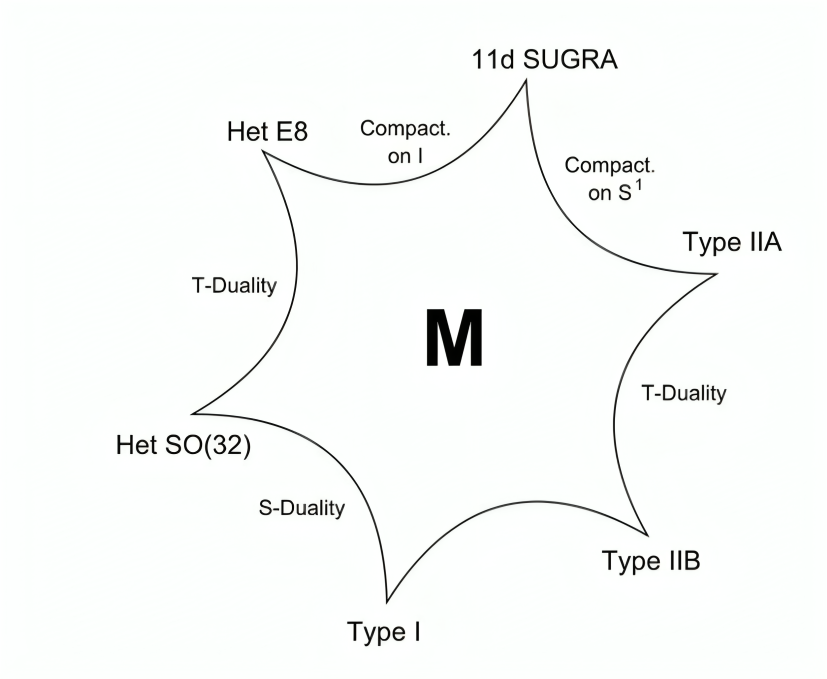
\includegraphics[width=0.6\textwidth]{Duality_star.png}
\caption{\small Schematic depiction of the web of dualities relating the different superstring theories in ten dimensions among each other, as well as to 11d M-theory.}
\label{fig:dualitystar}
\end{center}
\end{figure}
%%%%%%%%%%%

\subsection{Duality symmetries with lower supersymmetry}\label{ss:dualitieswithlowersusy}

As it was early realized, the existence of string dualities is actually a very generic phenomenon which is not tied to the high level of supersymmetry of our starting superstring theories in ten dimensions. In fact, the duality web described in the previous section rapidly grows both in broadness and complexity once we start considering non-trivial compactifications to lower spacetime dimensions. 

Here we will only comment on those symmetries which persist (or arise) when the compactification process breaks some of the original supersymmetries of the theory. In particular, and with an eye to future applications, we will pay special attention to string dualities that appear in 4d $\mathcal{N}=2$ settings.
 
\subsubsection*{Type IIA/Heterotic duality}

The first duality in lower dimensions that we want to discuss here involves the Type II and the $\mathsf{E8}\times \mathsf{E8}$ Heterotic strings. However, it is useful to argue for this using an intermediate relation between M-theory and Heterotic string theory in one dimension higher, since this will also appear at several instances of the thesis. 

Let us thus consider M-theory compactified on a $K3$ surface. As already discussed in Section \ref{sss:MtheoryonK3}, this leads to a seven-dimensional theory preserving 16 supercharges, whose moduli space is classically exact and is moreover described, in general, by the space of Ricci-flat metrics on $K3$. The latter exhibits a group coset structure of the form
%
\begin{align}\label{eq:modspaceK3surfaces}
	\mathcal{M}_{\text{K3}} = \mathsf{O(\Gamma_{3,19})}\backslash \mathsf{O(3,19)} / (\mathsf{O(3)} \times \mathsf{O(19))} \times \mathbb{R}_+\, ,
\end{align}
%
where the precise meaning of the different mathematical objects involved is discussed around eq. \eqref{eq:cosetspace7d}, and the $\mathbb{R}_+$ factor accounts for the overall $K3$ volume --- which belongs to the gravity multiplet. Crucially, the exact same moduli space arises when compactifying the Heterotic string on a flat 3-torus. This can be easily seen by recalling that the (Narain) moduli space of string theory compactifications on $k$-dimensional tori $\mathbf{T}^k$, when accounting for the full set of T-duality transformations, is indeed isomorphic to \cite{Narain:1985jj,Narain:1986am}
%
\begin{align}
	\mathcal{M}_{\mathbf{T}^k} = \mathsf{O(\Gamma_{k,k})}\backslash \mathsf{O(k,k)} / (\mathsf{O(k)} \times \mathsf{O(k))} \times \mathbb{R}_+\, ,
\end{align}
%
where the extra factor $\mathbb{R}_+$ is now associated to the 7d string coupling constant $g_7$. Hence, since the Heterotic string (in its bosonized description) includes 16 additional directions in e.g., the right-moving sector --- parametrizing a 16d compact torus with fixed radius of the order of the string scale, the resulting moduli space for $k=3$ indeed matches the one shown in \eqref{eq:modspaceK3surfaces}. Furthermore, taking into account that the graviton-dilaton piece of the Heterotic string action reads as
%
\begin{equation}
			\begin{aligned}
				S_\text{Het}^{\text{7d}} \, \supset\, &\frac{1}{2\kappa_{7}^2} \int \text{d}^{10}x\sqrt{-g} \left(\mathcal{R}-\frac{4}{5}(\partial \varphi_7)^2\right)\, , 
			\end{aligned}
\end{equation}
%
and upon comparing with \eqref{eq:7dMthyK3}, we deduce the following moduli identification
%
\begin{align}
\label{eq:mthyHetmoduli}
 g_7 = \mathcal{V}_{K3}^{3/4}\, , 
\end{align}
%
which relates the Heterotic string coupling constant with the overall internal volume in the M-theory frame. This means, in turn, that the small $K3$ limit, as seen from M-theory, would correspond to a weak coupling regime for a dual Heterotic string, which arises from a solitonic M5-brane wrapping the entire $K3$ surface,\footnote{Note that the tension of both objects agree exactly upon using the identification \eqref{eq:mthyHetmoduli}, namely
\begin{align}
 \notag \frac{T_{\text{M5, str}}}{M_{\text{Pl};\, 7}^2} = (4\pi)^{-2/5}\, \mathcal{V}_{K3}^{3/5} = (4\pi)^{-2/5}\,  g_7^{4/5} = \frac{T_{\text{het}}}{M_{\text{Pl};\, 7}^2}\, . 
\end{align}} whereas the strong $g_7$ limit (from the Heterotic point of view), induces some full decompactification to 11d M-theory instead. All this suggests that in fact both theories might be S-dual to each other, and indeed there exist by now multiple non-trivial checks of the proposed duality
%
\begin{align}\label{eq:duality7dMthHet}
\text{M-theory on}\; K3 \qquad \stackrel{\text{dual}}{\longleftrightarrow} \qquad \text{Heterotic string on}\; \mathbf{T}^3\, , 
\end{align}
%
see e.g., \cite{Witten:1995ex,Cherkis:1997bx,Park_2009} for an incomplete list of references.

Interestingly, one can propagate the above relation to theories living in lower dimensions and with less amount of supersymmetry as well. Doing so requires from considering M-theory on e.g., some $K3$-fibered Calabi--Yau thereefold, where the $K3$ is adiabatically fibered over a rational $\mathbb{P}^1$ curve, which should be much larger than the fibre itself. This allows us to perform the duality \eqref{eq:duality7dMthHet} \emph{fiberwise}, thus yielding the following relation between 5d $\mathcal{N}=1$ theories
%
\begin{align}\label{eq:duality5dMthHet}
\text{M-theory on}\; X_3 \cong K3\rightarrow \mathbb{P}^1 \qquad \stackrel{\text{dual}}{\longleftrightarrow} \qquad \text{Heterotic string on}\; K3 \times \mathbf{S}^1\, , 
\end{align}
%
where the internal space in the Heterotic side of the duality arises by fibering a $\mathbf{T}^2$ inside the $\mathbf{T}^3$ over the $\mathbb{P}^1$ base, which famously gives rise to a $K3$ surface.\footnote{Indeed, the K3 two-fold is known to have a locus on its moduli space where it arises as an elliptic fibration over a one-fold base $\mathbb{P}^1$ \cite{Weigand:2010wm}.}

Finally, let us mention that upon further compactification on $\mathbf{S}^1$, and by employing M-theory/Type IIA duality (c.f. eq. \eqref{IIAMduality}), one can argue for the existence of the following third S-dual relation \cite{Hull:1994ys,Ferrara:1995yx,Kachru:1995wm} (see \cite{Aspinwall:1996mn} for a comprehensive review)
%
\begin{align}\label{eq:IIA/HETduality4d}
\text{Type IIA on}\; X_3 \cong K3\rightarrow \mathbb{P}^1 \qquad \stackrel{\text{dual}}{\longleftrightarrow} \qquad \text{Heterotic string on}\; K3\times \mathbf{T}^2\, , 
\end{align}
%
where now it is the limit of large $\mathbb{P}^1$ volume (on the Type IIA side) the one corresponding to a weak coupling point for the dual Heterotic string, i.e. $g_4\rightarrow 0$. We will heavily make use of the above chain of dualities when discussing several important aspects studied in this thesis, see Chapters \ref{ch:Higherdimops}, \ref{ch:Emergence} and \ref{ch:pattern}.

\subsubsection*{M-/F-theory duality}

Let us discuss now one of the most interesting string dualities that have been derived so far. It relates in a highly non-trivial way the physics of M-theory with a non-perturbative description of Type IIB string theory (denoted F-theory) --- i.e. including D-branes, and in fact it is precisely via this duality how many phenomenologically viable scenarios have been constructed up to date within string theory, which are close to the Standard Model of Particle Physics (see e.g., \cite{Cvetic:2022fnv,Marchesano:2022qbx,Marchesano:2024gul} and references therein).

The crucial realization that motivated the development of F-theory was the intimate relation between the $\mathsf{SL(2,\mathbb{Z})}$ self-duality of Type IIB string theory (see discussion around eq. \eqref{eq:Sdualityrules10dIIB}) and the group of large diffeomorphisms of the torus, i.e. the modular transformations. The latter act solely on the complex structure of $\mathbf{T}^2$, such that one useful and very geometrical way to think about Type IIB string theory is to `embed' the description into some twelve-dimensional theory where two compact dimensions define some elliptic curve $\mathcal{C}$, with frozen volume and varying complex structure, as determined by the axio-dilaton profile $\tau (x)$ \cite{Vafa:1996xn}. However, the crucial insight is that this a priori auxiliary identification, does indeed have physical meaning via its connection to 11d M-theory, as we explain next.

Therefore, in order to establish the correspondence between F-theory and M-theory (or rather its 11d low-energy supergravity limit), we start by recalling that M-theory compactified on a circle $\mathbf{S}^1_a$ reduces to Type IIA string theory in the limit where the radius $R_a$ of the circle vanishes, namely when $R_a\rightarrow 0$. If we further reduce on an additional circle $\mathbf{S}^1_b$, one effectively arrives at a $\mathbf{T}^2$ compactification of M-theory, which after taking $R_a\rightarrow 0$, becomes Type IIA on $\mathbf{S}^1_b$. This is entirely equivalent to Type IIB on the T-dual circle $\overline{\mathbf{S}}^1_b$, with radius $\overline R_b =\alpha'/R_b$, as explained in Section \ref{ss:dualitieswithhighersusy}. Hence, by additionally approaching the small $R_b$ regime, we essentially decompactify $\overline R_b$ in Type IIB dual frame. Thus, we conclude that M-theory on $\mathbf{T}^2$ reduces to Type IIB string theory in the limit of vanishing torus volume, $\mathcal{V}_{\mathbf{T}^2}$, whereas the complex structure $\tau$ is left untouched. Additionally, one can see that the Kaluza-Klein tower associated to the decompactifying circle in the Type IIB frame corresponds, from the M-theory perspective, to M2-branes wrapping the whole torus-fibre $n \in \mathbb{Z}$ times, whose mass
%
\begin{align}\label{eq:massM2branes}
			m_{\text{M2}}\,  (n \mathbf{T}^2) = \left | \int_{n \mathbf{T}^2} J \right |= |n\, \mathcal{V}_{\mathbf{T}^2}|= \left |\frac{n}{\overline R_b} \right |\, ,    
\end{align}
%
goes then to zero in the limit $\overline R_b \to \infty$.
		
More generally, let us consider M-theory compactified on an elliptically-fibered $n$-fold $X_{n}$, over some $(n-1)$-fold base $C_{n-1}$, which we denote as follows
%
\begin{equation}\label{eq:fibration}
			\begin{aligned}
				\pi: \qquad \mathbf{T}^2 \hookrightarrow &\;X_{n} \\
				&\;\; \downarrow \qquad . \\ &\;C_{n-1}
			\end{aligned}
\end{equation}
%
One can then easily see that in order to preserve some unbroken supersymmetry in the low energy EFT, the $n$-fold needs to have at least vanishing first Chern class, i.e. it has to be Calabi--Yau  \cite{Denef:2008wq, Weigand:2010wm, Weigand:2018rez, Cvetic:2018bni}. This results in a supersymmetric EFT living in $\mathbb{R}^{1,10-2n}$. Performing now adiabatically the duality discussed above, namely by taking the limit of zero fibre volume from the M-theory perspective, one obtains Type IIB string theory compactified on $C_{n-1}$, possibly with some non-perturbative defects (i.e. 7-branes) wrapping certain cycles of the internal geometry (given by the singular loci of the torus fibration) \cite{Morrison:1996na,Morrison:1996pp}.

\subsubsection*{Mirror symmetry}

Finally, we turn to a fascinating property exhibited by certain 4d $\mathcal{N}=2$ theories, which is inherited from the simple T-duality relation described in Section \ref{ss:dualitieswithhighersusy} above. The proposal is to identify Type IIA and Type IIB string theories compactified on mirror (dual) Calabi--Yau manifolds. Let us briefly elaborate on this point. 

In fact, when discussing the low energy effective field descriptions arising from the aforementioned compactified theories (c.f. Section \ref{s:4dN=2}) it becomes readily apparent that they are essentially the same up to an exchange of the (extended) K\"ahler and complex structures (see e.g., \cite{Grimm:2005fa} for a review). This led originally \cite{Candelas:1989hd, Greene:1989cf,Greene:1990ud,Aspinwall:1990xe,Candelas:1990rm,Aspinwall_1994,kontsevich1994homological} to propose that (fully-fledged) Type IIA compactified on a CY three-fold $X_3$ is equivalent to (fully-fledged) Type IIB reduced on a different three-fold $Y_3$, satisfying 
%
\begin{align}
 h^{1,1}(X_3) = h^{2,1}(Y_3)\, ,\qquad h^{2,1} (X_3) = h^{1,1}(Y_3)\, ,
\end{align}
%
where the manifold $Y_3$ is usually referred to as the mirror of $X_3$. This implies, in turn, a
map between even-dimensional and middle-dimensional cohomologies on $X_3$ and $Y_3$, $H^{2p}(X_3) \leftrightarrow H^3(Y_3)$, with $p=0, \ldots,3$, and consequently, an analogous relation between integral, symplectic bases of the aforemetioned spaces
%
\begin{align}
\mathcal{C} \in H_{2p}(X_3) \longleftrightarrow \gamma \in H_{3}(Y_3)\, . 
\end{align}
%
The duality exchanging Type IIA on $X_3$ and Type IIB on $Y_3$ is referred to as \textit{(quantum) mirror symmetry},\footnote{The word quantum refers to the assertion that the full quantum string theories should be taken to be equivalent, which goes beyond the usual statement of the equivalence between the associated perturbative CFTs.} see \cite{Hori:2003ic,Hosono:1994av} for a detailed review on the topic. Therefore, applied to Type II string theories, this duality exchanges
%
\begin{align}\label{eq:mapmirrorsymmetry}
\mathcal{M}_{\text{VM}}^\text{IIA} \longleftrightarrow \mathcal{M}_{\text{VM}}^\text{IIB} \qquad \text{and} \qquad \mathcal{M}_{\text{HM}}^\text{IIA} \longleftrightarrow \mathcal{M}_{\text{HM}}^\text{IIB}\, . 
\end{align}
%
Notice that this implies that we can identify the \emph{quantum-corrected} K\"ahler moduli space $\mathcal{M}_{\text{QK}}$ pertaining to some three-fold $X_3$, with the \emph{classical} moduli space, $\mathcal{M}_{\text{CS}}$, of complex structures of the mirror manifold $Y_3$. We can hence identify e.g., the complexified K\"ahler moduli $\{z^a = b^a + \i t^a\}$ of Type IIA compactified on $X_3$ with the periods $\{Z^A\}$, used to describe the complex structure moduli space of Type IIB on $Y_3$, as follows
%
\begin{align}\label{mirrormap}
 z^a = \frac{Z^a}{Z^0}\, .
\end{align}
%
This is known as the mirror map. Notice, however, that Mirror Symmetry is \textit{a priori} defined in the large volume limit of $X_3$, i.e. $z^a \rightarrow \i \infty$, corresponding to the large complex structure limit of $Y_3$, i.e. $Z^a \rightarrow \i \infty$. This is due to the fact that the vector multiplet moduli space of Type IIA string theory receives $\alpha'$-corrections which are suppressed in this limit. On the other hand, the vector multiplet moduli space of Type IIB does not receive corrections of any sort and thus can be described in purely classical terms. Since the above duality states that the two moduli spaces need to be the same, the calculation of the periods $\{Z^A, \mathcal{F}_A\}$ of $Y_3$ can be actually used so as to infer $\alpha'$-corrections to the IIA moduli space, in particular worldsheet instanton contributions, see below. 

Close to the large complex structure point (LCS) of $Y_3$, one can find a basis of periods such that they split into a \textit{unique} power series plus single logs
%
\begin{align}\label{largecomplexperiods}
 Z^a = \frac{1}{2\pi \i } \log y^a + \mathcal{O}(y^a) \, ,\qquad Z^0 = 1 + \mathcal{O}(y^a)\, ,
\end{align}
%
with the large complex structure point corresponding to $y^a=0$. In practice it is a non-trivial task to find the correct basis of periods with this leading logarithmic behaviour, which is commonly referred to as integral basis. --- due to its properties under the (maximal unipotent) monodromies induced transforming the $y^a$-hyperplane as $y^a\rightarrow e^{2\pi \i }y^a$.

With this (rather special) basis one can now define inhomogeneous, flat coordinates on $\mathcal{M}_{\text{CS}}$ as follows 
%
\begin{align}\label{eq:coordinates}
 \tau^a = \frac{Z^a}{Z^0}=\frac{1}{2\pi \i } \log y^a + \mathcal{O}(y^a)\, ,
\end{align}
%
which coincide near $y=0$ with the classical complexified K\"ahler parameters $\tau^a (y \to 0) = b^a + \i t^a$ near the large volume limit of $X_3$. Away from $y=0$, the $\tau^a$ then define, via analytic continuation, the (multi-valued) coordinates over the full quantum K\"ahler moduli space, $\mathcal{M}_{\text{QK}}$.

From the periods \eqref{largecomplexperiods} one can then infer the prepotential $\mathcal{F}= (Z^{0})^2 F (z^a)$ that underlies the special K\"ahler geometry of the vector multiplet moduli space of Type IIA compactified on $X_3$ which takes the form
%
\begin{align}\label{prepotentialIIA}
F =-\frac{1}{6} \cK_{abc} z^a z^b z^c + K_{ab}^{(1)} z^a z^b + K_{a}^{(2)} z^a + K^{(3)} - \frac{1}{(2 \pi \i)^3}\sum_{\boldsymbol{k}\geq \boldsymbol{0}} n_{\boldsymbol{k}}^{(0)} \sum_{m \geq 1} \frac{1}{m^3} e^{2\pi \i m k_a z^a}\, , 
\end{align} 
%
where in terms of a dual basis $\lbrace \omega_a \rbrace$ of $H^2(X_3, \mathbb{Z})$ we have
%
\begin{align}
 \cK_{abc}= \omega_a \cdot \omega_b \cdot \omega_c \, ,\qquad K_{a}^{(2)}=\frac{1}{24} c_2(X_3) \cdot \omega_a\, ,\qquad K^{(3)}= \frac{\i \zeta(3)}{2(2\pi)^3} \chi_E(X_3)\, .
\end{align}
%
The $K_{ab}^{(1)}$ are in general not specified geometrically but can be determined (up to monodromy \cite{deWit:1992wf,Harvey:1995fq}) by requiring good symplectic transformation properties of the period vector
%
\begin{align}
    \Pi(z) &= \begin{pmatrix}
           Z^{0} \\
           Z^{a} \\
           \partial_a \mathcal{F} \\
           \partial_0 \mathcal{F}
         \end{pmatrix}=Z^{0} \begin{pmatrix}
           1 \\
           z^{a} \\
           \partial_a F \\
           2F- z^a \partial_a F
         \end{pmatrix}\, .
  \end{align}
%
Note that already the perturbative $\alpha'$-corrections in \eqref{prepotentialIIA} break, in general, the no-scale structure of the classical K\"ahler potential (c.f. eq. \eqref{eq:kahlersectormetric}). Thus, the term given by $K^{(3)}$ encodes contributions which descend from $\alpha'^3 \mathcal{R}^4$ curvature corrections already present in the 10d supergravity action (see e.g., \cite{Green:1999pv, Palti:2008mg,Grimm:2017okk}), and it turns out to be the only effective perturbative contribution to the K\"ahler potential $K_{\rm ks}$. As opposed to this, the terms $K_{ab}^{(1)}$ and $K_{a}^{(2)}$ correspond respectively to one-loop and two-loop corrections in $\alpha'$, yet do not have a ten-dimensional counterpart due to the lack of a ten-dimensional curvature polynomial with the appropriate features. Their presence is however physically irrelevant at the level of the K\"ahler metrics\cite{Escobar:2018rna},\footnote{However, both $K_{ab}^{(1)}$ and $K_{a}^{(2)}$ do appear in the 4d effective action \eqref{eq:IIAaction4d} through the kinetic and topological terms for the $\mathsf{U(1)}$ gauge fields determined by eq. \eqref{eq:holomorphicgauge kineticfunction4d} (see e.g., Appendix B of \cite{Marchesano:2022axe}).} as confirmed by their absence in the K\"ahler potential that results from \eqref{prepotentialIIA}
%
\begin{align}\label{eq:alpha'correctedKahlerpot}
 K_{\rm ks}=- \log \left(\frac{4}{3}\mathcal{K} +4 \i K^{(3)}\right)\, .
\end{align}
%
On the other hand, the non-perturbative terms in \eqref{prepotentialIIA} correspond to worldsheet instanton contributions to the prepotential, and can be deduced from the corrections to the periods that are polynomial in the $y^a$ (c.f. eq. \eqref{eq:coordinates}). There, $\boldsymbol{k}$ denotes a vector of length $h^{1,1}(X_3)$ that scans over positive homology classes $k_a\gamma^a \in H_2^+(X_3,\mathbb{Z})$. The coefficients $n_{\boldsymbol{k}}^{(0)}$ are known as genus-zero Gopakumar--Vafa invariants and count the BPS degeneracy of (bound states of) D2-branes wrapped on cycles in the homology class $k_a \gamma^a$\cite{Gopakumar:1998ii, Gopakumar:1998jq}.

Finally, as promised at the beginning of this subsection, let us stress that a useful way to think about Mirror Symmetry is via some particular chain of T-dualities \cite{Strominger:1996it}. In fact, this can be shown very explicitly in toroidal orbifold models, where upon explicitly performing three T-dualities via the familiar Bushcer rules (c.f. eqs. \eqref{eq:BuscherrulesNS}-\eqref{eq:BuscherrulesRR}) one arrives precisely at the map \eqref{eq:mapmirrorsymmetry}, see e.g., \cite{Ibanez:2012zz} for details. 

\section{The Swampland program} \label{s:SwamplandProgram}

In previous sections we have discussed various possibilities for low energy effective field theories that string or M-theory allows us to construct. These may differ in the number of non-compact spacetime dimensions --- depending on the internal manifold we place our theory on, the type and amount of gauge symmetries exhibited by the effective description (i.e. supersymmetry, non-Abelian interactions, etc.), or even the matter content. This diversity creates an enormous set of physically distinct vacua, which are collectively known as the \emph{String Landscape} \cite{Susskind:2003kw}. Crucially, all these theories share the common feature that can be embedded in string theory, and thus are compatible (by construction) with an ultra-violet completion of gravity. 

Historically though, the mere existence of this rich structure of vacua was considered to be detrimental for the theory, since it suggested that essentially every semi-classically consistent EFT that one may think of could be found within some corner of the String Landscape. Hence, trying to understand any physics beyond the Standard Model of Particle Physics using a top-down approach was regarded to be meaningless, since the theory did not seem to have any predictive power at all. However, as pointed out in \cite{Vafa:2005ui}, it turns out that coupling generic effective field theories to gravity can introduce certain inconsistencies --- which go beyond the usual gravitational anomaly analysis \cite{Alvarez-Gaume:1983ihn} --- that are not visible form the field theory prism. In fact, it is the aim of the \emph{Swampland Program} \cite{Vafa:2005ui} to delineate the boundary between the set of EFTs that can be derived from quantum gravity/string theory (thereby belonging to the Landscape) and those that are not consistent with gravitational interactions at a deeper level (referred to as the Swampland). 

The pursuit of distinguishing these two sets of effective field theories involves establishing definite criteria that any consistent EFT must satisfy in order to belong to the Landscape. In this regard, even though string theory plays a prominent role for uncovering universal constraints in quantum gravity, the idea of the Swampland can be formulated regardless of the former. In fact, heuristic arguments based on black hole physics can also contribute significantly to this discourse, providing insights which should be a priori independent of any underlying microscopic theory of quantum gravity. For instance, the \emph{no global symmetries conjecture} states that in a consistent theory of quantum gravity there cannot be exact global (continuous or discrete) symmetries \cite{Israel:1967za,Zeldovich:1976vq,Kallosh:1995hi,Susskind:1995da,Banks:1988yz, Banks:2010zn,Yonekura:2020ino}.\footnote{See e.g., \cite{Polchinski:1998rr} for a proof in string perturbation theory as well as \cite{Harlow:2018jwu, Harlow:2018tng} for an analogous statement AdS holographic spacetimes.} (See also \cite{McNamara:2019rup} for a more refined version of the conjecture including higher-form topological charges as well.) This can be motivated by studying black holes, which are singular solutions in general relativity that are independent of any global charge present in the theory \cite{Israel:1967za}, therefore leading to various puzzles in relation to charge conservation and the finiteness of the black hole entropy \cite{Bekenstein:1972tm,Hawking:1975vcx}. Remarkably, all these problems can be easily resolved once we preclude any conserved global charge from existing in the first place. Despite this, string theory remains a crucial testing ground for verifying the applicability of any proposed Swampland condition, as well as for exploring the intricate relationships and structures that underpin all these criteria. 

One of the main objectives of this thesis will be to understand the precise role that the quantum gravity cut-off $\LQG$, here understood as the energy scale where semi-classical Einstein gravity --- coupled to any sort of matter --- breaks down completely, plays within the Swampland program. In particular, we would like to study how it behaves in generic effective theories of gravity, so as to ensure the fulfillment of these quantum gravity (or Swampland) constraints, and hopefully extract some general and useful lessons. To do so, we will restrict ourselves to string theory constructions mostly in flat spacetime backgrounds, although many of the considerations applied in this work could be in principle extended to other approaches of quantum gravity such as holography, via the AdS/CFT correspondence  \cite{Maldacena:1997re,Witten:1998qj}. For reasons that will become more apparent as we progress in the thesis, we will be particularly interested in two conjectures: the Distance Conjecture and the Weak Gravity Conjecture. They are both introduced and discussed in detail in Sections \ref{s:SDC} and \ref{s:WGC}, respectively. For an in-depth review of these and other Swampland conjectures, we refer the reader to the comprehensive discussions that can be found in \cite{Brennan:2017rbf,Palti:2019pca,vanBeest:2021lhn,Grana:2021zvf,Harlow:2022gzl,Agmon:2022thq,VanRiet:2023pnx}.

\subsection{The Weak Gravity Conjecture}\label{s:WGC}

The Weak Gravity Conjecture (WGC) was originally proposed in \cite{Arkani-Hamed:2006emk} and subsequently studied in many follow up works, resulting in several generalizations and refinements thereof (see \cite{Palti:2020mwc, Harlow:2022gzl} for some recent reviews on this conjecture and related ideas). Here we will focus on a formulation of the conjecture for $\mathsf{U(1)}$ gauge theories, see however \cite{Heidenreich:2017sim} for a discussion involving non-abelian gauge groups and product groups as well. There are in fact two versions of the original conjecture:\footnote{We focus here in the four-dimensional formulation. Note that the factors and the powers of the Planck mass would change in different dimensions \cite{Heidenreich:2015nta}, and we will include them explicitly when dealing with cases where $d \neq 4$, see e.g., Chapter \ref{ch:Emergence}.} 
%
\begin{itemize}
\item[] \textbf{Electric Weak Gravity Conjecture:} 
In a $\mathsf{U(1)}$ gauge theory coupled to gravity there must exist a charged state of mass and charge given by $\{m, q\}$, respectively, and whose charge-to-mass ratio is \emph{superextremal}, i.e. 
%
\begin{align}\label{WGCel}
 \frac{q^2 g^2}{m^2} \geq \left. \frac{Q_{\rm BH}^2 g^2}{M_{\rm BH}^2}\right|_{\text{ext}}\, ,
\end{align}
%
where the right hand side of the inequality refers to the charge-to-mass ratio of a extremal black hole in the theory, and $g$ denotes the gauge coupling constant. 
\item[] \textbf{Magnetic Weak Gravity Conjecture:} 
For a $\mathsf{U(1)}$ gauge theory coupled to gravity, there exists an upper bound for the UV cut-off $\Lambda_{\rm EFT}$ of the effective field theory, which is given by 
%
\begin{align}\label{WGCmag}
\Lambda_{\rm EFT} \leq g \Mpf\, . 
\end{align}
%
\end{itemize}
%
The importance of this conjecture lies in the fact that it attempts to make sharp statements about the charged spectrum of a $\mathsf{U(1)}$ gauge theory coupled to Einstein gravity. For instance, one direct implication of the condition \eqref{WGCel} is that pure Einstein-Maxwell gravity without matter (valid all the way up to $\Mpf$) must belong to the Swampland. As for the magnetic version, notice that it can be motivated in two different ways. One can either apply the electric version \eqref{WGCel} to the Hodge dual field strength $\tilde{F} = \star F$, thus forcing the theory to have a \emph{magnetic monopole} whose mass $m_{\rm mon}$ is smaller than its (physical) charge, or rather it can be recovered by directly imposing that the theory has some monopole that is not yet a black hole state. The EFT would then break down at energies close to $\Lambda_{\rm EFT} \approx m_{\rm mon}$, because it is there where it becomes sensitive to the monopole degrees of freedom, which can no longer be treated as solitonic objects.

For concreteness, let us consider Einstein-Maxwell theory coupled to a massive charged scalar $\phi$ in 4d, with an action that reads (at leading order)
%
\begin{equation}
\label{eq:EinsteinMaxwell}
S_{\mathrm{EM}}=\int \dd^{4} x \sqrt{-g}\left(\frac{1}{2 \kappa_4^2}\, \mathcal{R}-\frac{1}{4 g^{2}} F^{2} - \overline{D_\mu \phi} D^\mu \phi - m^2 |\phi|^2 \right)\, ,
\end{equation}
%
where the covariant derivative is defined as follows
%
\begin{equation}
D_\mu \phi= \left(\partial_\mu + \i q A_\mu \right) \phi\, , \qquad q \in \IZ\, .
\end{equation}
%
To get a grasp on what the conjecture is telling us, let us try to understand what goes wrong from the gravitational physics perspective when e.g., eq. \eqref{WGCmag} is not satisfied. Notice that the global\footnote{The global part of a gauge symmetry group $G$ (as well as the so-called large gauge transformations) is strictly speaking not included in the definition of a global symmetry (when $g$ is finite), since there is no gauge invariant charged local operator $\mathcal{O}(x)$ that is acted non-trivially by $G$ (see \cite{vanBeest:2021lhn} for more details).} part of this gauge symmetry acts on the field as
%
\begin{equation}\label{eq:globalpartsymm}
\phi \rightarrow e^{2\pi \i q \alpha} \phi\, ,
\end{equation}
%
with $\alpha$ being any constant parameter. Hence, if we insist on taking the limit $g\rightarrow 0$ we can actually recover an exact $\mathsf{U(1)}$ global symmetry, since the gauge boson $A_{\mu}$ decouples, such that \eqref{eq:globalpartsymm} survives as a remnant. To prevent this pathological behaviour from happening, the regime of validity of the EFT must shrink to zero size (in energies), which is precisely what eq. \eqref{WGCmag} imposes. Let us remark, though, that the above arguments are merely heuristic considerations. Nevertheless, as already commented at the beginning of this section, they serve the purpose of illustrating some of the universal ideas behind quantum gravity, which ultimately lead to non-trivial constraints which can be motivated independently of string theory. On the other hand, the Weak Gravity Conjecture is actually supported by a rich amount of top-down constructions within string theory, and its connection to the no-global symmetries proposal can be made much more rigorous, see e.g, \cite{Harlow:2018jwu, Harlow:2018tng,Montero:2018fns}.

Let us also comment here that an alternative, and perhaps more insightful, viewpoint on the Weak Gravity Conjecture is to interpret the latter as imposing that there should not be stable charged black hole remnants, which requires in turn to ask that the self-interaction of the state with highest charge-to-mass ratio is repulsive. This condition is usually referred to as the Repulsive Force Conjecture \cite{Palti:2017elp,Heidenreich:2019zkl, Lee:2018spm}, and roughly speaking it requires gravity to provide for the \emph{weakest} force (which is precisely the behaviour observed in Nature), namely
%
\begin{align}\label{CoulombGrav}
 |\vec{F}_\text{Coulomb}|  \geq |\vec{F}_\text{grav}| \Longleftrightarrow \frac{q^2 g^2}{m^2} \geq \frac{1}{\Mpd^{d-2}} \frac{d-3}{d-2}\, ,
\end{align}
%
precisely reducing to \eqref{WGCel} when $d=4$.\footnote{See also \cite{Palti_2017,Lee:2018spm,Gonzalo:2019gjp,Gonzalo:2020kke} for further extensions so as to include attractive Yukawa-like interactions as well.}

Let us finally introduce certain classes of refinements of the WGC which will play an important role in later parts of this thesis, also in connection with the Distance Conjecture discussed in Section \ref{s:SDC} below. Up to now, we have only asked for the theory to contain a \emph{single} (possibly very massive) state whose charge-to-mass ratio is superextremal. However, there exist various versions of the conjecture which indeed ask for the presence of an \emph{infinite} number of states --- with increasing mass --- satisfying \eqref{WGCel} instead \cite{Cheung:2014vva, Heidenreich:2015nta, Heidenreich:2016aqi,Montero:2016tif}. The rationale for this would be the requirement to have a stable statement under dimensional reduction (thereby including additional gauge fields that can appear in the compactification process, such as the Kaluza-Klein photon). This motivates tower \cite{Andriolo:2018lvp} and/or sub-Lattice versions of the WGC \cite{Heidenreich:2015nta, Heidenreich:2016aqi}, which have been tested up to date with an impressive level of accuracy in all known string theory compactifications, see e.g., \cite{Lee:2018urn,Lee:2019tst,Lee:2019skh,Lee:2019xtm,Heidenreich:2019bjd,Klaewer:2020lfg,Alim:2021vhs,Heidenreich:2021yda,Gendler:2022ztv,Cota:2022yjw,Cota:2022maf,Heidenreich:2024dmr} for an incomplete list of references.\footnote{See however \cite{Cota:2023uir} for a recent alternative statement that does not always impose the necessity of having an infinite number of superextremal particle states.}

\subsection{The Distance Conjecture}\label{s:SDC}

The Distance Conjecture \cite{Ooguri:2006in}, on the other hand, articulates some conjectural behaviour concerning effective gravitational theories characterized by some moduli space $\mathcal{M}$. (See however \cite{Calderon-Infante:2020dhm} for extensions and checks in theories lacking a quantum exact moduli space.) As already mentioned, this space is parameterized by the massless scalar fields within the theory, and it possesses a natural intrinsic metric defined by the kinetic terms associated to those.\footnote{Strictly speaking, the kinetic terms of the scalar fields are given by the pullback $f^*$ of the map $f: \mathbb{R}^{1, d-1} \to \mathcal{M}$ applied to the non-linear $\sigma$-model metric parameterizing the scalar manifold geometry $\mathcal{M}$, to the physical spacetime $\mathbb{R}^{1, d-1}$, whose coordinatization is given precisely by the scalar fields themselves.} The conjecture posits that, first of all, the diameter of the moduli space should be infinite, meaning that there should exist \emph{at least} one geodesic exploring infinite distance. Therefore, strictly compact moduli spaces, which are perfectly fine from the field theory point of view (for instance, one could simply consider Einstein gravity coupled to a massless and shift-symmetric scalar field $\theta \sim \theta + 2\pi$), should not be allowed in quantum gravity. Secondly, it states that, upon starting at some point $P \in \mathcal{M}$ and after traversing an infinite distance toward a second point $Q$ along some geodesic direction, one should encounter an infinite tower of states becoming light in Planck units. More precisely, this fall-off in the mass scale associated to the tower must be such that 
%
\begin{equation}
m_{\rm tow}(Q)\ \sim \ m_{\rm tow}(P) \ \, e^{-\lambda \,  d(P,Q)}\, , \qquad \text{as}\ \ d(P,Q)\rightarrow \infty\, ,
\label{eq:masslesstower}
\end{equation}
%
is satisfied, with $\lambda$ being some $\mathcal{O}(1)$ constant (in Planck units) that has been moreover conjectured to be greater than or equal to $\frac{1}{\sqrt{d-2}}$ \cite{Etheredge:2022opl}, where $d$ is the number of spacetime dimensions. Thus, at infinite distance, the effective field theory --- with dynamical gravity --- must break down due to the presence of an (infinite tower of) nearly massless states, which were not accounted for in the original EFT. This can be stated formally by saying that the naive effective field theory cut-off decreases exponentially with the moduli space distance, as follows
%
\begin{equation}
\Lambda_{\text{EFT}}(Q)\ \sim \ \Lambda_{\text{EFT}}(P) \ \, e^{-\lambda\,  d(P,Q)}\, ,
\end{equation}
%
where we have identified $\Lambda_{\text{EFT}} = m_{\rm tow}$ in the above equation. Notice that, strictly speaking, this does \emph{not} necessarily mean that a purely field-theoretic approach cannot be employed for energies well above $\Lambda_{\text{EFT}}$ (or $m_{\rm tow}$), since it may be possible to define some different local field theory description when e.g., the theory decompactifies and the tower verifying \eqref{eq:masslesstower} is comprised by Kaluza-Klein replica; for instance a higher-dimensional field theory. What it \emph{does} imply is the necessity of abandoning our original EFT construction.

A very simple realization of the Distance conjecture can be found when compactifying $d$-dimensional gravity on a circle of radius $R$. For concreteness, and in order to make contact with our discussion in Section \ref{s:maxsugraintro}, let us consider 11d supergravity on $\mathbf{S}^1$. Once we sit in the 10d Einstein frame, the scalar-gravitational sector of the theory reads as (c.f. eq. \eqref{eq:3formddimgravity})
%
\begin{equation}
	\label{eq:scalartensorMthonS1}
	\begin{aligned}
		S^{\text{10d}}_{\text{M-th}}\, \supset\ -\frac{1}{2\kappa_{10}^2} \int \dd^{10}x\sqrt{-g} \left(\mathcal{R}-\frac{9}{8}(\partial \rho)^2\right)\, ,
	\end{aligned}
\end{equation}
%
so that the moduli space of the theory corresponds to the possible v.e.v.s of the radius field $R= e^{\rho}$, whose metric has the form
%
\begin{align}
  G_{R R} = \frac{9}{8}\, \frac{1}{R^2}\, .
\end{align}
%
Therefore, the associated geodesic distance between any two values for the radius modulus, $R_i$ and $R_f$, is thus computed to be
%
\begin{equation}
d(R_i, R_f)=  \frac{3}{\sqrt{8}}\, \int_{R_i}^{R_f} \dfrac{\dd R}{R} =  \frac{3}{\sqrt{8}}\, \log \left( \frac{R_f}{R_i} \right)\, ,
\end{equation}
%
which presents two infinite distance points, namely at $R \to 0, \infty$. In the latter case, the limit corresponds to a decompactification back to eleven dimensions, where as already mentioned, it is the Kaluza-Klein states on the $\mathbf{S}^1$ the ones that become light at a rate
%
\begin{equation}
\frac{m_{\rm KK}}{M_{\text{Pl};\, 10}}=  (4\pi)^{-1/8}\, R^{-9/8} = (4\pi)^{-1/8}\, e^{-\frac{3}{\sqrt{8}}\, d(1,\, R)}\, ,
\end{equation}
%
hence exhibiting some $\lambda = \frac{3}{\sqrt{8}} \geq \frac{1}{\sqrt{8}}$. From this perspective, the Distance conjecture does not seem to impose any non-trivial requirement. Note, however, that this is not true anymore if probing the remaining infinite distance limit, i.e. $R \to 0$, where there seems to be a priori no field-theoretic degrees of freedom that can make \eqref{eq:masslesstower} hold. In fact, we already know what is the tower fulfilling the conjecture, since the small radius limit actually implements the duality with Type IIA string theory, whose fundamental object becomes weakly coupled precisely along this regime, such that we find
%
\begin{equation}
\frac{T_{\rm M2,\, str}}{M_{\text{Pl};\, 10}^2}=  (4\pi)^{-1/4}\, R^{3/4} \Longrightarrow \frac{m_{\rm tow}}{M_{\text{Pl};\, 10}} = \frac{m_s}{M_{\text{Pl};\, 10}} = (4\pi)^{-1/8}\, e^{-\frac{1}{\sqrt{8}}\, d(1,\, R)}\, ,
\end{equation}
%
where now $\lambda = \frac{1}{\sqrt{8}}$. This simple example gives us various important insights. First, the conjecture seems to require from additional ingredients beyond the original EFT description, namely extended objects, such as the M2-brane. Second, it also becomes intimately related with the concept of dualities in quantum gravity, as explained in Section \ref{s:dualities} above.

Let us stress here the fact that, despite the good amount of evidence gathered in favour of the conjecture (see e.g., \cite{Montero:2015ofa,Baume:2016psm,Klaewer:2016kiy,Valenzuela:2016yny,Blumenhagen:2017cxt,Palti:2017elp,Hebecker:2017lxm,Grimm:2018ohb,Heidenreich:2018kpg,Blumenhagen:2018nts,Landete:2018kqf,Lee:2018urn,Reece:2018zvv,Lee:2018spm,Ooguri:2018wrx,Grimm:2018cpv,Buratti:2018xjt,Hebecker:2018fln,Gonzalo:2018guu,Corvilain:2018lgw,Lee:2019tst,Blumenhagen:2019qcg,Joshi:2019nzi,Font:2019cxq,Lee:2019xtm,Grimm:2019wtx,Lee:2019wij, Erkinger:2019umg, EnriquezRojo:2020hzi,Gendler:2020dfp,Grimm:2020cda,Bastian:2020egp,Baume:2020dqd, Perlmutter:2020buo, Calderon-Infante:2020dhm,Grimm:2020ouv, Ooguri:2024ofs,Aoufia:2024awo,Lanza:2020qmt, Lanza:2021udy, Lanza:2022zyg} for an incomplete set of references), there is still no completely satisfactory microscopic argument explaining why it should hold in general, even though currently there are some interesting proposals trying to address this point (see Chapter \ref{ch:Emergence} for more on this).\footnote{See \cite{Rudelius:2024vmc} for recent arguments based on generalized symmetries.}

\subsubsection*{Emergent String Conjecture}

One simple yet important question that the previous analysis raises concerns the type of (lightest) towers that can appear upon exploring infinite distance limits in quantum gravitational field spaces. Indeed, already in the example mentioned before, we saw two different kind of behaviours arising in our theory: either the former decompactifies and it is the Kaluza-Klein tower of states who furnish the Distance Conjecture, or rather we end up probing a tensionless limit for a (possibly dual) fundamental string (an emergent string limit). Hence, it is natural to wonder at this point whether there could be any other behaviour (i.e. different from the aforementioned ones), that could arise in quantum gravity at infinite distance; for instance, the appearance of some asymptotically tensionless membrane dominating the light spectrum of the theory. Indeed, this would be both striking and very interesting at the same time, since it could hint toward yet unknown UV completions of gravity not involving strings at all. 

However, in \cite{Lee:2019wij} the authors proposed that this observed pattern is in fact all that can actually occur in quantum gravity, such that there could not be any other possible UV complete theory arising at infinite distance. This conjecture is referred to as the Emergent String Conjecture, and states that any equi-dimensional infinite distance limit\footnote{\label{fnote:equidimensional}Here equi-dimensional means that the asymptotic physics is governed by a theory defined in the same number of space-time dimensions as the original theory in the interior of the moduli space.} needs to correspond to some infinite distance point in moduli space where a critical string becomes tensionless and weakly coupled. Therefore, along these degenerations the tower of states predicted by \eqref{eq:masslesstower} comprise the excitations of the light, critical string (c.f. eq. \eqref{eq:modeexpansionclosedstring}-\eqref{eq:fermionmodeexpansionstrings}). Interestingly, as argued in \cite{Alvarez-Garcia:2021pxo}, consistency of the Emergent String Conjecture under dimensional reduction seems to forbid e.g., membrane limits where it is a fundamental 2-brane which dominates the light spectrum of the theory.

Crucially, there seems be always a \textit{unique} critical string becoming tensionless at the fastest rate, such that in principle no two different massless gravitons can arise in the spectrum of light states.
